\documentclass[journal]{IEEEtran}

\usepackage{cite}
\usepackage{amsmath,amssymb,amsfonts}
\usepackage{algorithmic}
\usepackage{graphicx}
\usepackage{textcomp}
\usepackage{subfig}
\usepackage{float}
\usepackage{xcolor}
\def\BibTeX{{\rm B\kern-.05em{\sc i\kern-.025em b}\kern-.08em
    T\kern-.1667em\lower.7ex\hbox{E}\kern-.125emX}}

\ifCLASSINFOpdf
  % \usepackage[pdftex]{graphicx}
  % declare the path(s) where your graphic files are
  % \graphicspath{{../pdf/}{../jpeg/}}
  % and their extensions so you won't have to specify these with
  % every instance of \includegraphics
  % \DeclareGraphicsExtensions{.pdf,.jpeg,.png}
\else
  % or other class option (dvipsone, dvipdf, if not using dvips). graphicx
  % will default to the driver specified in the system graphics.cfg if no
  % driver is specified.
  % \usepackage[dvips]{graphicx}
  % declare the path(s) where your graphic files are
  % \graphicspath{{../eps/}}
  % and their extensions so you won't have to specify these with
  % every instance of \includegraphics
  % \DeclareGraphicsExtensions{.eps}
\fi
% graphicx was written by David Carlisle and Sebastian Rahtz. It is
% required if you want graphics, photos, etc. graphicx.sty is already
% installed on most LaTeX systems. The latest version and documentation
% can be obtained at: 
% http://www.ctan.org/pkg/graphicx
% Another good source of documentation is "Using Imported Graphics in
% LaTeX2e" by Keith Reckdahl which can be found at:
% http://www.ctan.org/pkg/epslatex
%
% latex, and pdflatex in dvi mode, support graphics in encapsulated
% postscript (.eps) format. pdflatex in pdf mode supports graphics
% in .pdf, .jpeg, .png and .mps (metapost) formats. Users should ensure
% that all non-photo figures use a vector format (.eps, .pdf, .mps) and
% not a bitmapped formats (.jpeg, .png). The IEEE frowns on bitmapped formats
% which can result in "jaggedy"/blurry rendering of lines and letters as
% well as large increases in file sizes.
%
% You can find documentation about the pdfTeX application at:
% http://www.tug.org/applications/pdftex





% *** MATH PACKAGES ***
%
%\usepackage{amsmath}
% A popular package from the American Mathematical Society that provides
% many useful and powerful commands for dealing with mathematics.
%
% Note that the amsmath package sets \interdisplaylinepenalty to 10000
% thus preventing page breaks from occurring within multiline equations. Use:
%\interdisplaylinepenalty=2500
% after loading amsmath to restore such page breaks as IEEEtran.cls normally
% does. amsmath.sty is already installed on most LaTeX systems. The latest
% version and documentation can be obtained at:
% http://www.ctan.org/pkg/amsmath





% *** SPECIALIZED LIST PACKAGES ***
%
%\usepackage{algorithmic}
% algorithmic.sty was written by Peter Williams and Rogerio Brito.
% This package provides an algorithmic environment fo describing algorithms.
% You can use the algorithmic environment in-text or within a figure
% environment to provide for a floating algorithm. Do NOT use the algorithm
% floating environment provided by algorithm.sty (by the same authors) or
% algorithm2e.sty (by Christophe Fiorio) as the IEEE does not use dedicated
% algorithm float types and packages that provide these will not provide
% correct IEEE style captions. The latest version and documentation of
% algorithmic.sty can be obtained at:
% http://www.ctan.org/pkg/algorithms
% Also of interest may be the (relatively newer and more customizable)
% algorithmicx.sty package by Szasz Janos:
% http://www.ctan.org/pkg/algorithmicx




% *** ALIGNMENT PACKAGES ***
%
%\usepackage{array}
% Frank Mittelbach's and David Carlisle's array.sty patches and improves
% the standard LaTeX2e array and tabular environments to provide better
% appearance and additional user controls. As the default LaTeX2e table
% generation code is lacking to the point of almost being broken with
% respect to the quality of the end results, all users are strongly
% advised to use an enhanced (at the very least that provided by array.sty)
% set of table tools. array.sty is already installed on most systems. The
% latest version and documentation can be obtained at:
% http://www.ctan.org/pkg/array


% IEEEtran contains the IEEEeqnarray family of commands that can be used to
% generate multiline equations as well as matrices, tables, etc., of high
% quality.




% *** SUBFIGURE PACKAGES ***
%\ifCLASSOPTIONcompsoc
%  \usepackage[caption=false,font=normalsize,labelfont=sf,textfont=sf]{subfig}
%\else
%  \usepackage[caption=false,font=footnotesize]{subfig}
%\fi
% subfig.sty, written by Steven Douglas Cochran, is the modern replacement
% for subfigure.sty, the latter of which is no longer maintained and is
% incompatible with some LaTeX packages including fixltx2e. However,
% subfig.sty requires and automatically loads Axel Sommerfeldt's caption.sty
% which will override IEEEtran.cls' handling of captions and this will result
% in non-IEEE style figure/table captions. To prevent this problem, be sure
% and invoke subfig.sty's "caption=false" package option (available since
% subfig.sty version 1.3, 2005/06/28) as this is will preserve IEEEtran.cls
% handling of captions.
% Note that the Computer Society format requires a larger sans serif font
% than the serif footnote size font used in traditional IEEE formatting
% and thus the need to invoke different subfig.sty package options depending
% on whether compsoc mode has been enabled.
%
% The latest version and documentation of subfig.sty can be obtained at:
% http://www.ctan.org/pkg/subfig




% *** FLOAT PACKAGES ***
%
%\usepackage{fixltx2e}
% fixltx2e, the successor to the earlier fix2col.sty, was written by
% Frank Mittelbach and David Carlisle. This package corrects a few problems
% in the LaTeX2e kernel, the most notable of which is that in current
% LaTeX2e releases, the ordering of single and double column floats is not
% guaranteed to be preserved. Thus, an unpatched LaTeX2e can allow a
% single column figure to be placed prior to an earlier double column
% figure.
% Be aware that LaTeX2e kernels dated 2015 and later have fixltx2e.sty's
% corrections already built into the system in which case a warning will
% be issued if an attempt is made to load fixltx2e.sty as it is no longer
% needed.
% The latest version and documentation can be found at:
% http://www.ctan.org/pkg/fixltx2e


%\usepackage{stfloats}
% stfloats.sty was written by Sigitas Tolusis. This package gives LaTeX2e
% the ability to do double column floats at the bottom of the page as well
% as the top. (e.g., "\begin{figure*}[!b]" is not normally possible in
% LaTeX2e). It also provides a command:
%\fnbelowfloat
% to enable the placement of footnotes below bottom floats (the standard
% LaTeX2e kernel puts them above bottom floats). This is an invasive package
% which rewrites many portions of the LaTeX2e float routines. It may not work
% with other packages that modify the LaTeX2e float routines. The latest
% version and documentation can be obtained at:
% http://www.ctan.org/pkg/stfloats
% Do not use the stfloats baselinefloat ability as the IEEE does not allow
% \baselineskip to stretch. Authors submitting work to the IEEE should note
% that the IEEE rarely uses double column equations and that authors should try
% to avoid such use. Do not be tempted to use the cuted.sty or midfloat.sty
% packages (also by Sigitas Tolusis) as the IEEE does not format its papers in
% such ways.
% Do not attempt to use stfloats with fixltx2e as they are incompatible.
% Instead, use Morten Hogholm'a dblfloatfix which combines the features
% of both fixltx2e and stfloats:
%
% \usepackage{dblfloatfix}
% The latest version can be found at:
% http://www.ctan.org/pkg/dblfloatfix




%\ifCLASSOPTIONcaptionsoff
%  \usepackage[nomarkers]{endfloat}
% \let\MYoriglatexcaption\caption
% \renewcommand{\caption}[2][\relax]{\MYoriglatexcaption[#2]{#2}}
%\fi
% endfloat.sty was written by James Darrell McCauley, Jeff Goldberg and 
% Axel Sommerfeldt. This package may be useful when used in conjunction with 
% IEEEtran.cls'  captionsoff option. Some IEEE journals/societies require that
% submissions have lists of figures/tables at the end of the paper and that
% figures/tables without any captions are placed on a page by themselves at
% the end of the document. If needed, the draftcls IEEEtran class option or
% \CLASSINPUTbaselinestretch interface can be used to increase the line
% spacing as well. Be sure and use the nomarkers option of endfloat to
% prevent endfloat from "marking" where the figures would have been placed
% in the text. The two hack lines of code above are a slight modification of
% that suggested by in the endfloat docs (section 8.4.1) to ensure that
% the full captions always appear in the list of figures/tables - even if
% the user used the short optional argument of \caption[]{}.
% IEEE papers do not typically make use of \caption[]'s optional argument,
% so this should not be an issue. A similar trick can be used to disable
% captions of packages such as subfig.sty that lack options to turn off
% the subcaptions:
% For subfig.sty:
% \let\MYorigsubfloat\subfloat
% \renewcommand{\subfloat}[2][\relax]{\MYorigsubfloat[]{#2}}
% However, the above trick will not work if both optional arguments of
% the \subfloat command are used. Furthermore, there needs to be a
% description of each subfigure *somewhere* and endfloat does not add
% subfigure captions to its list of figures. Thus, the best approach is to
% avoid the use of subfigure captions (many IEEE journals avoid them anyway)
% and instead reference/explain all the subfigures within the main caption.
% The latest version of endfloat.sty and its documentation can obtained at:
% http://www.ctan.org/pkg/endfloat
%
% The IEEEtran \ifCLASSOPTIONcaptionsoff conditional can also be used
% later in the document, say, to conditionally put the References on a 
% page by themselves.




% *** PDF, URL AND HYPERLINK PACKAGES ***
%
%\usepackage{url}
% url.sty was written by Donald Arseneau. It provides better support for
% handling and breaking URLs. url.sty is already installed on most LaTeX
% systems. The latest version and documentation can be obtained at:
% http://www.ctan.org/pkg/url
% Basically, \url{my_url_here}.

 \newcommand{\commentrenan}[1] {\textcolor{blue}{[RL: #1]}}



% *** Do not adjust lengths that control margins, column widths, etc. ***
% *** Do not use packages that alter fonts (such as pslatex).         ***
% There should be no need to do such things with IEEEtran.cls V1.6 and later.
% (Unless specifically asked to do so by the journal or conference you plan
% to submit to, of course. )


% correct bad hyphenation here
\hyphenation{op-tical net-works semi-conduc-tor}


\begin{document}
%
% paper title
% Titles are generally capitalized except for words such as a, an, and, as,
% at, but, by, for, in, nor, of, on, or, the, to and up, which are usually
% not capitalized unless they are the first or last word of the title.
% Linebreaks \\ can be used within to get better formatting as desired.
% Do not put math or special symbols in the title.
\title{Development of a Novel Retrofit Framework Considering Industry 4.0 Concepts: A Case Study of a Didactic Manufacture Production System}
%
%
% author names and IEEE memberships
% note positions of commas and nonbreaking spaces ( ~ ) LaTeX will not break
% a structure at a ~ so this keeps an author's name from being broken across
% two lines.
% use \thanks{} to gain access to the first footnote area
% a separate \thanks must be used for each paragraph as LaTeX2e's \thanks
% was not built to handle multiple paragraphs
%

\author{Rafael~da~Silva~Mendonca, %%~\IEEEmembership{Member,~IEEE,}
        Renan~Landau~Paiva~de~Medeiros,~\IEEEmembership{Member,~IEEE,}
        and~Vicente~Ferreira~de~Lucena~Jr.,~\IEEEmembership{Senior~Member,~IEEE}% <-this % stops a space
\thanks{This research, carried out within the scope of the Samsung-UFAM Project for Education and Research (SUPER), according to Article 39 of Decree n°10.521/2020, was funded by Samsung Electronics of Amazonia Ltda., under the terms of Federal Law n°8.387/1991 through agreement 001/2020, signed with UFAM and FAEPI, Brazil. The authors thank the scholarship and financial support in part by the FAPEAM, CAPES, CNPq, and UFAM.}}% <-this % stops a space
% \thanks{J. Doe and J. Doe are with Anonymous University.}% <-this % stops a space
% \thanks{Manuscript received April 19, 2005; revised August 26, 2015.}}

% note the % following the last \IEEEmembership and also \thanks - 
% these prevent an unwanted space from occurring between the last author name
% and the end of the author line. i.e., if you had this:
% 
% \author{....lastname \thanks{...} \thanks{...} }
%                     ^------------^------------^----Do not want these spaces!
%
% a space would be appended to the last name and could cause every name on that
% line to be shifted left slightly. This is one of those "LaTeX things". For
% instance, "\textbf{A} \textbf{B}" will typeset as "A B" not "AB". To get
% "AB" then you have to do: "\textbf{A}\textbf{B}"
% \thanks is no different in this regard, so shield the last } of each \thanks
% that ends a line with a % and do not let a space in before the next \thanks.
% Spaces after \IEEEmembership other than the last one are OK (and needed) as
% you are supposed to have spaces between the names. For what it is worth,
% this is a minor point as most people would not even notice if the said evil
% space somehow managed to creep in.



% The paper headers
\markboth{Journal of \LaTeX\ Class Files,~Vol.~14, No.~8, August~2015}%
{Shell \MakeLowercase{\textit{et al.}}: Bare Demo of IEEEtran.cls for IEEE Journals}
% The only time the second header will appear is for the odd numbered pages
% after the title page when using the twoside option.
% 
% *** Note that you probably will NOT want to include the author's ***
% *** name in the headers of peer review papers.                   ***
% You can use \ifCLASSOPTIONpeerreview for conditional compilation here if
% you desire.




% If you want to put a publisher's ID mark on the page you can do it like
% this:
%\IEEEpubid{0000--0000/00\$00.00~\copyright~2015 IEEE}
% Remember, if you use this you must call \IEEEpubidadjcol in the second
% column for its text to clear the IEEEpubid mark.



% use for special paper notices
%\IEEEspecialpapernotice{(Invited Paper)}




% make the title area
\maketitle

% As a general rule, do not put math, special symbols or citations
% in the abstract or keywords.
\begin{abstract}

Retrofitting legacy systems provides significant advantages by addressing compatibility issues with new devices and technologies, meeting current process requirements, and enhancing security and regulatory compliance. The process starts with collecting requirements and evaluating the legacy system's attributes and limitations, followed by integrating new technologies to improve efficiency, streamline processes, and enhance performance and interoperability while leveraging existing facilities to reduce costs. A systematic approach ensures updates align with modern technological standards, with performance evaluations conducted using qualitative and quantitative methods, and system maturity assessed according to the RAMI model's criteria for intelligent factories. By incorporating Digital Twin (DT) capabilities, which replicate the physical state of systems and provide real-time data updates, the retrofit strategy aligns the physical system with Industry 4.0 contexts, facilitating continuous improvement and seamless integration with modern processes. The ultimate goal is to technologically advance the legacy system to ensure seamless integration with contemporary processes, validated through RAMI criteria analysis for smart factories.

\end{abstract}

% Note that keywords are not normally used for peerreview papers.
\begin{IEEEkeywords}
methodology, retrofitting, legacy system, digital twin, RAMI 4.0 and smart factory criteria.
\end{IEEEkeywords}



% For peer review papers, you can put extra information on the cover
% page as needed:
% \ifCLASSOPTIONpeerreview
% \begin{center} \bfseries EDICS Category: 3-BBND \end{center}
% \fi
%
% For peerreview papers, this IEEEtran command inserts a page break and
% creates the second title. It will be ignored for other modes.
\IEEEpeerreviewmaketitle
% Bajic~\cite{Bajic2021} and Ahmed~\cite{Ahmed2022}  define the main technologies, characteristics, and implementations related to I4.0 and define that the main purpose is to connect all aspects of the production process and create an integrated, adaptable, and autonomous system.


\section{Introduction}

\IEEEPARstart{T}{he} digital twin (DT) is widely used in Industry 4.0 (I4.0) to increase process efficiency and flexibility, improve quality, and increase reliability through the use of various technologies. It allows the process and its assets to be monitored and managed in real time, identifying possible problems and opportunities before they occur and helping the decision process.

Bajic~\cite{Bajic2021} and Ahmed~\cite{Ahmed2022} delineate the core technologies and implementations of I4.0, emphasising its goal of integrating all facets of production into an adaptable, autonomous system. Key technologies include the Internet of Things (IoT)~\cite{Garg2020}, cloud computing (CC)~\cite{Mahmud2020}, cyber-physical system (CPS)~\cite{Fraga2020, Sinha2020}, and big data (BD)~\cite{Nguyen2020, Qi2018}. Among these technologies, digital twin (DT)~\cite{Schroeder2021} emerged as a virtual counterpart to physical objects or processes, permitting the simulation and replication of real-world behaviours. Constructed from real-time data, DTs support simulations, monitoring, predictions, and optimizations, effectively aligning with I4.0 objectives.

Researchers conceive of digital twins (DTs) as a mechanism facilitating synchronization between physical and virtual twins, thus enabling seamless integration of both realms~\cite{Wanasinghe2020, Turner2021}. The representation of the product life cycle within DTs encapsulates real-world actions alongside their virtual counterparts, incorporating operational data, actuators, and sensors~\cite{Mihai2022}. A DT capacity to reflect real-time updates from physical assets ensures the continuous enhancement of virtual models, thereby facilitating system simulation, monitoring, analysis, and decision support.

DTs can reproduce the system’s state and update data in real-time, continuously improving virtual models based on physical assets' behaviour. Through DT, system simulation and monitoring become achievable, enabling analysis, diagnostics, and decision-making support. This capability allows legacy systems to be efficiently and economically updated to leverage the benefits of the industry 4.0 paradigm. The proposed architecture aims to update and enhance system processes while integrating the physical system with a virtual model for continuous monitoring to improve performance evaluation.

The efficiency of the architecture will be evaluated using both qualitative and quantitative methods, with the system’s maturity assessed based on the RAMI reference model~\cite{Bastos2021, Alemao2022, Lopez2023}. The objective is to ensure that the updated system operates at peak performance and meets current and future industry demands.

Based on data from the literature~\cite{Ooi2020, Mendonca2023}, this study contributes to the development of a retrofit methodology targeted at digital twin implementation, facilitating the creation of a virtual model for the updated system. Retrofitting~\cite{Tran2022, Li2024} entails the update to more contemporary and advanced components. The authors introduce their concept of retrofitting a legacy system~\cite{Carrillo2023}, defined as the process of updating a system, typically aimed at enhancing its performance, safety, or functionality. The goal is to integrate technologies, rendering the legacy system technologically proficient enough to interact and integrate with current systems. Specifically, the chosen case study revolves around updating a legacy system—a system originally designed and implemented using outdated technologies that may no longer suffice for actual industrial needs, especially those aligned with modern standards.

There are several reasons why applying retrofitting to a legacy system is advantageous. For instance, legacy systems may lack compatibility with new devices or technologies, or they may fail to meet current process requirements~\cite{annett2019}. Additionally, the legacy system might be susceptible to security threats or may not comply with prevailing standards or regulations. Hence, the procedure commences with the collection of requirements from the legacy system and the evaluation of its attributes and limitations. Subsequently, it involves the adoption of new technologies for integration, enhancing efficiency, and streamlining the process, with a focus on achieving improved system performance and interoperability~\cite{gao2019}. Moreover, it provides an economical solution by leveraging existing facilities and equipment, thereby reducing investment costs.

The step-by-step implementation of the retrofit process aims to furnish a systematic and structured approach to updating legacy systems~\cite{seacord2001}. It involves identifying updated requirements, defining objectives, and making assumptions for development. Consequently, the procedural guide delineates a clear and concise pathway for retrofitting legacy systems. By adhering to the outlined steps, systematic updates can be made to existing systems, ensuring alignment with modern technological requirements. Subsequently, the performance of the updated legacy system will undergo evaluation utilizing both qualitative and quantitative methods. Additionally, the system's maturity will be gauged based on the levels of maturity stipulated in the RAMI model\cite{ding2022}, considering its criteria for smart factories.

Enhancing the alignment of the physical system with Industry 4.0 contexts, the strategy for updating a legacy system in manufacturing aims at efficient and economical enhancement. Digital twin (DT) capabilities enable the replication of the systems' physical state (physical twin) and real-time data updates, thereby facilitating the continuous improvement of virtual models (digital twins) based on updates from physical assets. Consequently, the DT architecture serves as a complementary tool within the proposed retrofit framework for legacy systems. 

In essence, the goal is to integrate technologies, rendering the legacy system sufficiently technologically advanced to integrate seamlessly with other processes. In this context,  validation entails analysis to ascertain the maturity of the RAMI and determine the current level of the updated system. The evaluation will be based on the application of criteria for smart factories.

\section{Proposed Retrofit Framework}
\label{sec:dt_retro}

\begin{figure*}[]
	\centering
	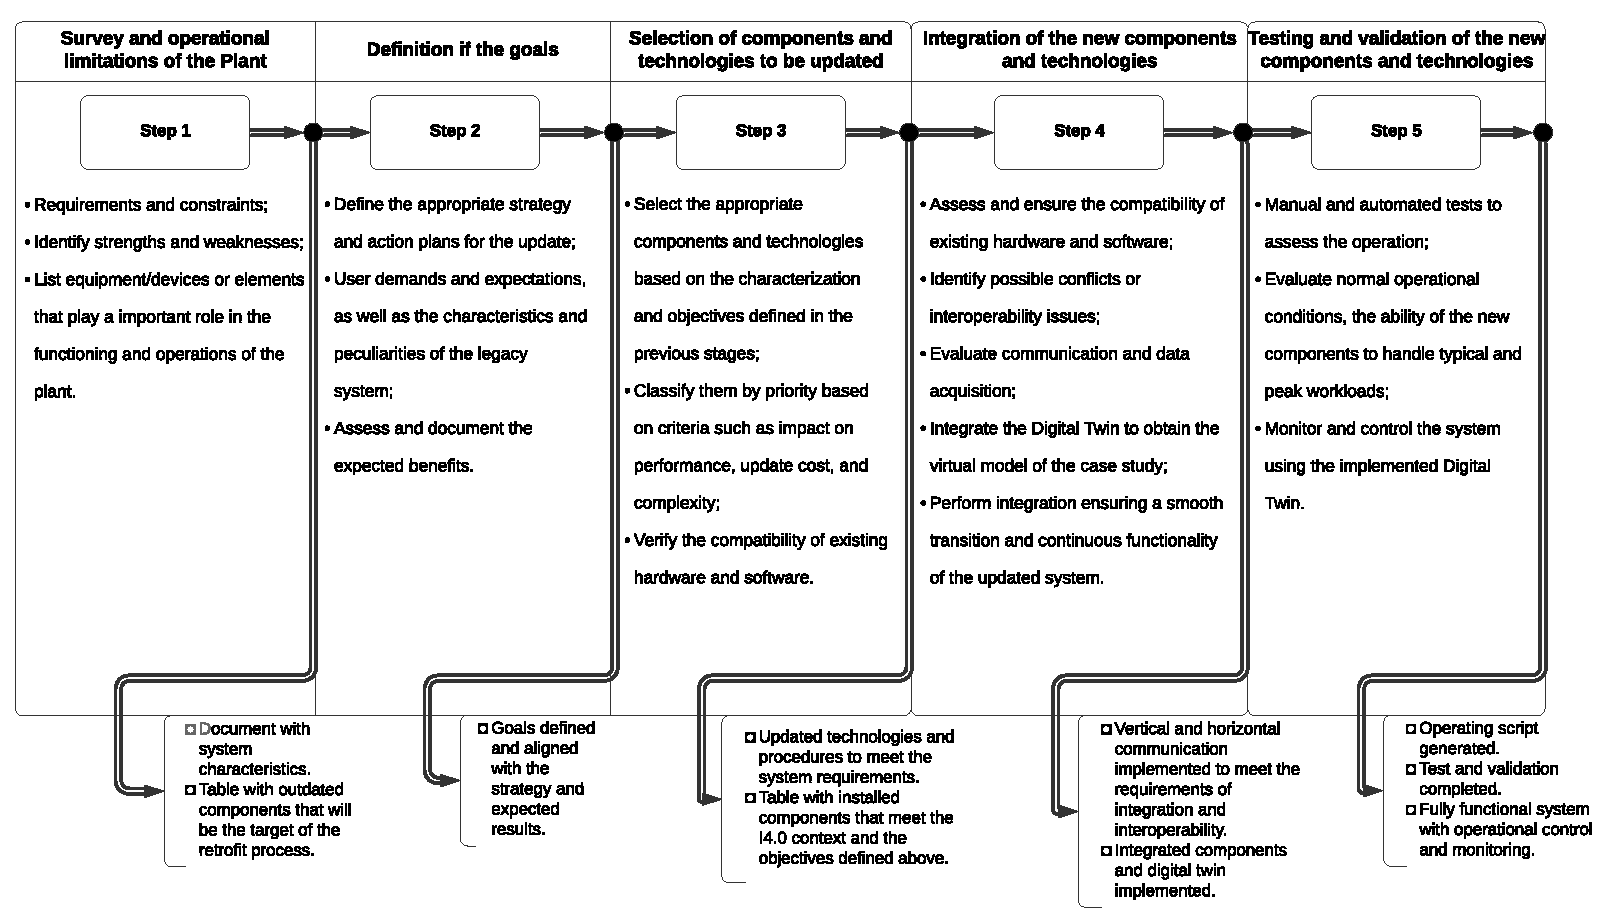
\includegraphics[width=0.99\linewidth]{figuras/flow_pretrofit_f.pdf}
	\caption{ General step diagram of the proposed retrofitting framework}
	\label{fig:metodology_diagram}
\end{figure*}

To update a legacy system using retrofit techniques, it is necessary to follow a well-defined process that can start with the identification and establishment of update goals, to improve efficiency, reduce costs, enhance quality, strengthen security, and meet other desirable objectives.
 
Retrofitting, as described by~\cite{Garcia2020} and~\cite{Niemeyer2020}, is an approach that aims to update existing systems or production processes. The main purpose is to make them more efficient, flexible, secure, and adaptable to new needs and technologies. This procedure may include adding or replacing devices or technologies, as well as integrating information or management systems as needed.

In parallel, conducting a thorough analysis of the legacy system is important. This analysis involves identifying the legacy system's devices, dependencies, interactions, problems, and limitations. This enables the appropriate selection of technologies that will be used in the update. These technologies consider the updated goals as well as the specific characteristics of the legacy system.

During the update process, it is worth defining the devices, procedures, and processes that will be the target of modification. After, tests must be done to ensure correct functioning, with the necessary adjustments made when problems are identified. Additionally, it is essential to provide training to users so that they can interact effectively with the implemented changes.

Based on the state-of-the-art, the proposed retrofit framework is developed by using the following steps to identify problems and consolidate modernization. Figure~\ref{fig:metodology_diagram} presents a general diagram that outlines the flow of stages to be applied to successfully achieve the proposed retrofit framework. Each step is detailed in the following section. 

\subsection{STEP 1 - Survey and operational limitations of the plant} 

To ensure successful retrofitting, conducting a detailed analysis of the existing legacy system is important. This involves identifying its strengths and weaknesses, as well as its requirements and constraints. Figure~\ref{fig:metodology_flow}a depicts a diagram outlining the flow of this stage and the expected outcome, taking into account factors, such as evaluating individual components and the technologies that need to be updated or replaced; expected benefits, potential risks and impacts; cost estimation; and establishing implementation timelines, among others.

By considering all these aspects, it is possible to make decisions about which components to update and how to proceed with the update. This stage is highly important because it provides the foundation for all subsequent steps. Therefore, the precise and detailed completion of this stage is fundamental for a successful updating process, beginning with a thorough understanding of the plant, environment, and/or installation where the legacy system is deployed. This understanding takes the form of diagrams, schematics, operation flowcharts, and relevant documentation.

Hence, with this information, equipment and devices, or elements that play a role in the plant's operation activities are identified. Consequently, these assets may be the primary targets for an update, regardless of the component's condition (whether it has deteriorated) or the need for an update (if it falls under legacy technology).

\subsection{STEP 2 - Definition of goals}

To define the appropriate strategy and action plans for the update, it is important to identify the goals for updating the legacy system, which may include improving efficiency, reducing costs, and increasing flexibility. Figure~\ref{fig:metodology_flow}b illustrates a diagram outlining the flow of this stage and the expected outcome, emphasizing the identification of the goals and considering user needs and expectations, as well as the characteristics and peculiarities of the legacy system. It is also important to assess the expected benefits, risks, and impacts, among other aspects.

In addition to defining the goals, it is relevant to evaluate and document the expected benefits resulting from the successful implementation of the \textit{retrofit} process. This may include cost reduction, increased productivity, fewer failures, improved energy efficiency, and sustainability.

The definition of solid and realistic goals and mapping the constraints of the legacy system are essential for effectively guiding the retrofitting process. These goals provide a road map for project decisions, goal fulfilment, and successful assessment. Therefore, careful consideration of the identified needs the evaluation of benefits and risks, and mapping the constraints of the legacy system and impacts help ensure that the update meets established expectations and quality standards.

\subsection{STEP 3 - Selection of Components and Technologies to be Updated}

To ensure a successful updating process, it is important to select appropriate components and technologies based on the previous characterization and defined goals. Figure~\ref{fig:metodology_flow}c illustrates a diagram outlining the flow of this stage and the expected outcome based on the selection of which components or technologies will be updated; their prioritization is based on criteria such as impact on performance, update cost, and installation complexity.

Maintaining a consistent alignment between the decisions made at the initiation stage and throughout the entire retrofitting process is important. This alignment is essential in ensuring that all actions taken are in line with the specific requirements of the plant. For example, by carefully choosing the components and technologies that are compatible with the existing systems, you can significantly mitigate integration and operational issues that could arise from incompatibility. This compatibility ensures a smoother transition during the retrofitting process.

The alignment also allows for foresight in technology selection, ensuring that the chosen technologies can be easily updated or expanded in the future. This step is vital in maintaining the system's relevance and adaptability over time, reducing the need for further extensive retrofits. Therefore, the selection of appropriate components and technologies is a fundamental aspect of the retrofitting process. The impact of these choices can greatly influence the overall effectiveness and success of the project.

\subsection{STEP 4 - Integration of New Components and Technologies}

Before proceeding with the integration, it is essential to assess the compatibility of the new components and technologies with the legacy system. This includes identifying potential conflicts, interoperability issues, and hardware and software requirements. The compatibility of communication protocols is also relevant for ensuring effective communication between systems. Figure~\ref{fig:metodology_flow}d illustrates a diagram outlining the flow of this stage and the expected outcome.

\begin{figure*}[!h]
	\centering
	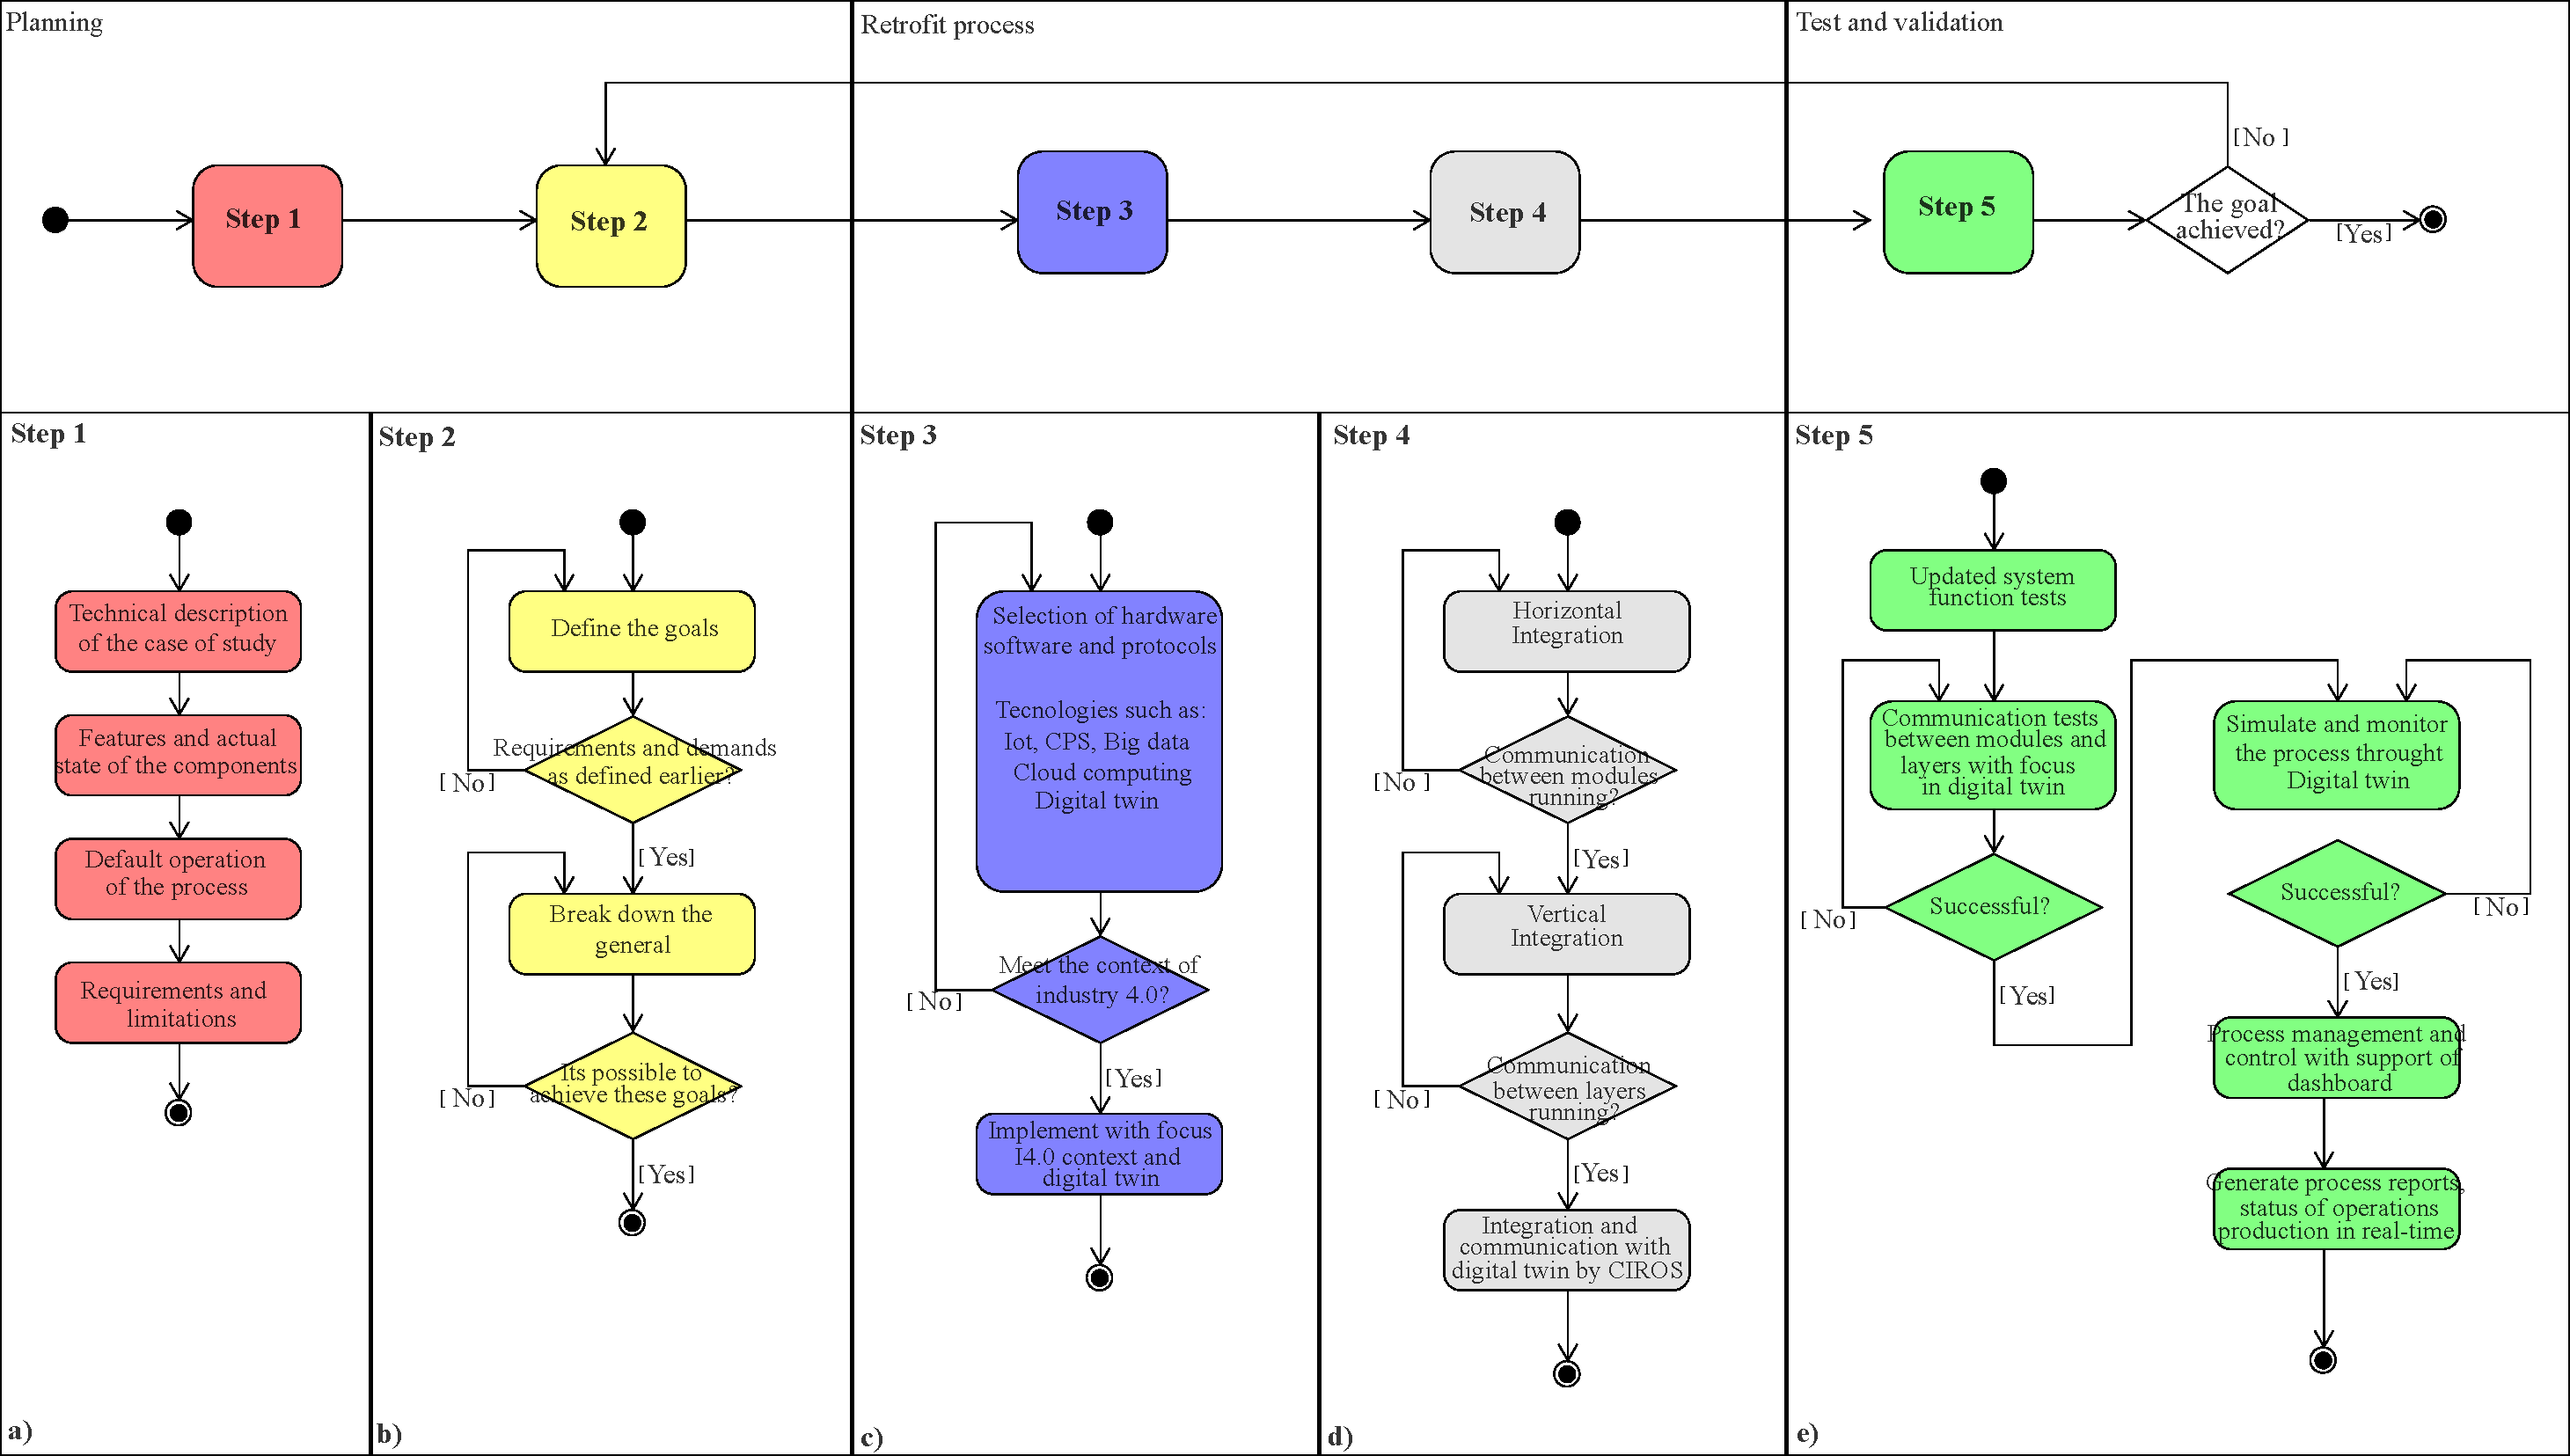
\includegraphics[angle=00, width=0.97\linewidth]{figuras/flow_final.pdf}
	\caption{ Flowchart of the proposed retrofit framework}
	\label{fig:metodology_flow}
\end{figure*}

Therefore, in this stage, it is important to use a detailed integration plan that outlines the necessary steps to incorporate the new components into the existing system, and the sequence of activities, schedules, and procedures for the tests that will be conducted in the next stage.

Integration tests are carried out with careful attention to detail to establish the appropriate operation of the new components and validate the success of their integration. This procedure involves looking at the combined operation of all system components to identify any compatibility issues or communication breakdowns.

These tests are designed not just to guarantee that each part functions properly, but also to ensure that they perform together harmoniously. Any concerns that develop during testing can be resolved quickly, resulting in a smoother transition and lowering the possibility of operational disruptions afterwards.

\subsection{STEP 5 - Testing and Validation of New Components and Technologies}

A combination of human and automated tests is an excellent technique for evaluating the capabilities of new components and technologies. Manual tests use a hands-on approach, with functionalities evaluated and confirmed manually, whereas automation tests allow for efficient repetition of usage situations, increasing the overall scope of tests.

As shown in Figure~\ref{fig:metodology_flow}e, this stage of the process involves conducting specific tests. These tests have the goal of assessing the system under normal operational settings, measuring the new components' ability to manage both typical and peak workloads, and assessing how well the new components integrate into the old system.

Simulation is used to develop scenarios that test the performance of new components under various conditions without interfering with the system's actual operations. This creates a safe setting for identifying and addressing any difficulties.

The testing and validation process plays an important role in ensuring that improvements to the legacy system are implemented smoothly and that previously specified goals are accomplished. This stage provides a crucial opportunity to detect and resolve issues before they affect regular operations.

This contributes significantly to the continuous integrity and functionality of the modified system. This procedure serves not only as a quality gatekeeper but also as a protection for the system's long-term performance and stability.

\subsection{Outlook and expected results of the proposal}

The primary purpose of using a retrofit methodology is to update and improve legacy systems, bringing them following a more modern context. Continuous monitoring and preventive maintenance become more important as these systems maturity, even when updates are applied. This emphasizes the importance of continuous operational monitoring, performing scheduled and corrective maintenance, and replacing components as needed.

\begin{figure*}[ht]
	\centering
	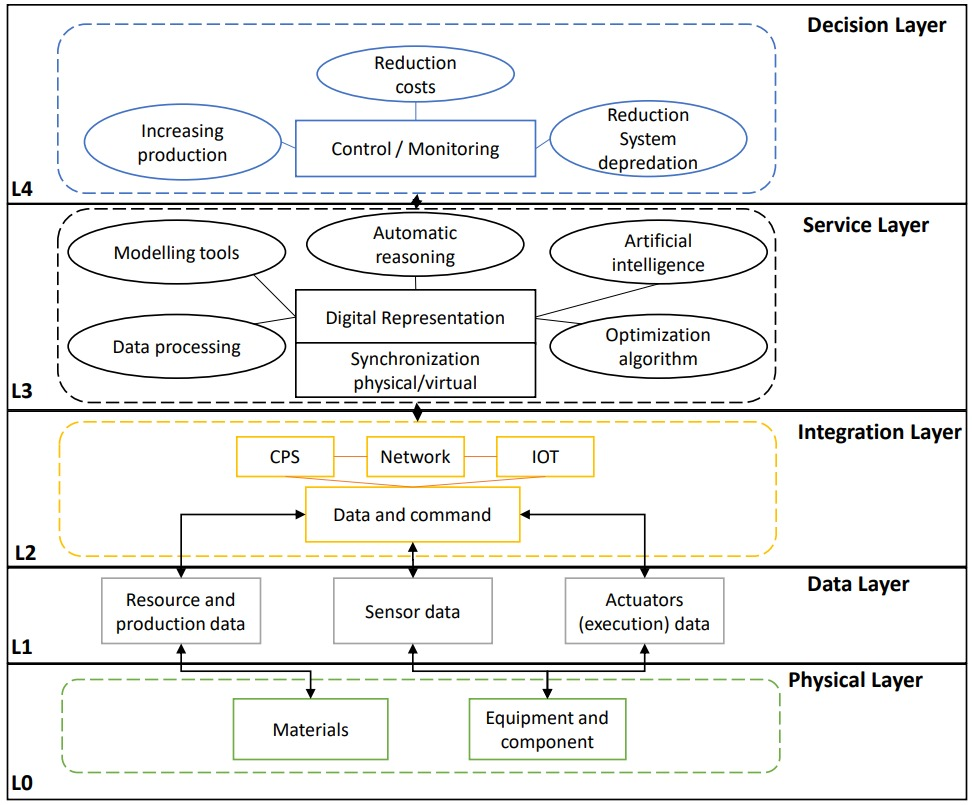
\includegraphics[width=0.94\linewidth]{figuras/arch_final.jpeg}
	\caption{Architecture of digital twin~\cite{Mendonca2022}.}
	\label{fig:arch_retro}
\end{figure*}

The retrofit procedure is supposed to increase efficiency as the system benefits from a succession of enhancements caused by the introduction of new technology and components. These updates can increase processing speed while decreasing processing time and downtime.

Another predicted effect of the retrofit procedure is enhanced security. New technologies frequently include advanced security features, such as two-factor authentication and data encryption, which add an extra layer of safety to the system.

The retrofit also increases the system's flexibility. New technology can make the system more adaptable to present and future changes or demands. This adaptability is essential in today's fast-changing technology environment. Furthermore, the retrofitting process might lead to lower maintenance expenses. New components and technology are frequently easier to maintain and update, resulting in significant long-term cost reductions.

Finally, the five-step process outlines a structured plan for doing a retrofit in a legacy system. This plan guarantees that updates are deployed successfully, preserving the system's integrity and operation while also accomplishing project goals.

\section{Architecture of the digital twin}

The implementation of this research was based on the proposed architecture inspired by the RAMI 4.0 model presented in previous works by Mendonca~\cite{Mendonca2022} and, as shown in Figure~\ref{fig:arch_retro}, the architecture was divided into layers, with the DT as the central element of the CPS. Each layer of the proposed architecture is presented in sequence to provide a comprehensive understanding of the structure of the CPS.

DTs serve as a support, for instance, to develop CPS by providing a unified platform for integrating and managing physical and information systems, enabling simulations and predictions, and optimizing the performance of the process\cite{Lopez2023b}. The proposed framework provides a structured approach to implementing DT and a global visualization of the interaction between layers and components of the process.
% The physical layer (L0)

\textbf{The physical layer (L0)} of the proposed architecture includes the physical elements of the Cyber-Physical System (CPS). These components include sensors, actuators, conveyors, robotic arms, and pumps. This layer is in charge of monitoring and collecting data from the physical devices.

Horizontal communication protocols like Profinet or Modbus make it easier to communicate between the many units in this layer. The data collected from these devices will be sent to the next layer, the data layer, for processing and management.

\textbf{The data layer (L1)} manages the constant flow of data from the physical layer. This includes data collected by devices, sensors, and actuators. At this layer, a variety of data-driven methodologies can be used to filter, classify, and organize data to be processed.

\textbf{The integration layer (L2)} is essential in providing fluid interaction between layers. It fills the gap between physical and virtual systems. This layer utilizes a variety of technologies, including the Internet of Things, to effectively link different systems and operations.

\textbf{The service layer (L3)} is important for the development of digital twins (DTs). It utilizes the integration provided by the layer below it (L2) to synchronize with the data and physical layers.

Monitoring, diagnosis and prognosis, verification and validation, fault identification, and management are just some of the services which digital twins can offer. They achieve this by applying data processing, modelling tools, automated reasoning, artificial intelligence (AI), and optimization algorithms.

\textbf{The decision layer (L4)} manages the structure of the system to achieve goals that are defined. These aims could involve improving production, minimizing system wear, and reducing production costs. To accomplish these goals, the decision layer can use communication protocols to vertically integrate the system.

One important feature of the decision layer is the ability to utilize a script, which can be done utilizing services such as process monitoring, control, or diagnosis. For example, a digital twin can provide failure prognosis services by evaluating a system device's remaining life and planning the replacement of devices, sensors, or other process components. This permits maintenance conditions to be changed to reduce costs (minimize losses), to extend the component's life while ensuring that the process runs continuously.

These five layers offer a structured approach for carrying out a retrofit in a legacy system. They guarantee that updates are carried out properly while maintaining the system's integrity and operation, as well as ensuring project objectives are met. The successful completion of a retrofit project results in considerable improvements in system performance, efficiency, and safety.

\subsection{Application}

The Digital Twin (DT) can integrate all layers of the proposed architecture, utilizing the capabilities of the Cyber-Physical System (CPS) to ensure complete control and operation of the entire process\cite{lee2020}. This is accomplished by modelling the operation on a virtual product life cycle model.

The suggested structure includes a variety of functionalities, each involving a distinct technology. These technologies can be integrated into the system in two ways: vertically or horizontally.

Vertical integration occurs at multiple layers of the architecture. It binds the layers together, allowing data and commands to flow seamlessly from top to bottom and vice versa~\cite{pisching2018}. For example, vertical integration allows sensors in the physical layer to communicate with applications in the service layer.

Horizontal integration, on the other hand, occurs at a single architectural layer~\cite{canas2022}. It entails creating communication between devices and systems that function on the same level. Horizontal integration, for example, could involve communication between multiple sensors in the physical layer.

Finally, the proposed structure offers a comprehensive and systematic approach to system integration, allowing for efficient management and operation of all parts of the process. The result is a more efficient, durable, and intelligent system that can meet the demands of today's manufacturing environments.

\subsection{Digital twin of the proposed retrofit framework}

Given its particular characteristics, the proposed retrofit procedure will incorporate the Digital Twin (DT) architecture. The DT operates as a real-time virtual representation of the system, allowing for the monitoring of sensor and actuator actions throughout the process.

Additionally, the DT enables the simulation and testing of potential updates before their actual implementation. This not only decreases the risks connected with system changes but also improves the retrofit process. 

% Figure~\ref{fig:arch_retro} illustrates how the retrofit method improved each layer of the DT design.

Interoperability concerns are common in systems that use components from multiple manufacturers, particularly when attempting to build communication interfaces across different modules and devices. However, the strategic combination of the suggested architecture and the implementation of the retrofit process effectively tackles these challenges, resulting in improvements at numerous levels:

\begin{itemize}
    \item Physical Layer: Improvements include new sensors, actuators, and protocols that improve hardware and communication.
    \item Data Layer: Sensor updates improve information collecting by ensuring a huge volume of data, pre-processing it (filtering or classifying), and transferring it to the integration layer (vertical integration).
    \item Integration and Service Layers: The update improves connection and vertical integration, particularly in the areas of information sharing and data collecting. These layers can communicate with the data and physical layers, allowing the development of DT, which provides services such as data processing and monitoring tools.
    \item Business Layer: This layer improves overall process management by supporting the other levels and improving decision-making.   
\end{itemize}

The connection of the service layer with legacy systems, as well as the specification of how data analysis and simulations will be performed using the DT, are equally important. To guarantee that the implementation is efficient and effective, all procedures should follow the best practices and standards specified by the proposed design, which is based on the Reference Design Model for Industries 4.0 (RAMI).

RAMI provides criteria for evaluating and validating outcomes related to the architecture's implementation and industry maturity level. These criteria permit the evaluation and categorization of the legacy system's digital transformation, as well as the measurement of the system's level of Industry 4.0 maturity after the update.

Furthermore, examining the system's maturity and criteria, as well as validating the use of the retrofit process, enables realistic evaluation of results. This technique highlights the modified system's Industry 4.0 characteristics, allowing for a more precise projection of the acquired result, efficacy, and alignment with the Industry 4.0 environment.

\subsection{Maturity Analysis based on the RAMI Model}

The analysis utilizing various criteria is an approach to measure the level of maturity and performance in accordance to the Reference Architecture Model for Industries 4.0 (RAMI)~\cite{ramos2020}. RAMI architecture integrates both quantitative and qualitative evaluations to evaluate the performance of manufacturing systems~\cite{hasbullah2023}.

The quantitative analysis is an objective evaluation that includes quantitative factors such as production volume and time, downtime, and incident reaction time, among others. This consists of total production, energy efficiency, and downtime of production systems. The analysis, which is based on numerical measures, aids in measuring the performance of production systems and creating goals. It is normally carried out by analysing data collected by components such as sensors and information systems. This allows for the measurement of key metrics for performance like utilization rate and production functionality.

In contrast, qualitative analysis is a subjective review that considers qualitative factors such as the quality of components, devices, systems, manufacturing processes, and generated information. Considering it depends on subjective assessments, it can be used to evaluate more subjective aspects of manufacturing systems, such as flexibility, agility, and product quality. This evaluation can be carried out through user interviews, production process observations, and document and report analysis.

In the context of RAMI architecture, it is desirable to integrate the two studies. This fusion enables a more precise and comprehensive assessment of the Industry 4.0 system or process, which helps in decision-making and manufacturing process optimization. Furthermore, these studies may assist in the planning and execution of updates and improvements.

To determine and categorize the system's level, it is required to evaluate the technique in the application and as an approach to ensure that smart factory criteria are met. The parameters and levels (ranging from 1 to 5) - A higher level represents a closer alignment with Industry 4.0.

The evaluation must be performed simultaneously at the start (to assess the legacy system) and at the end of the methodology application (the updated system). This comparison can be used as a reference to evaluate the improvements that occurred by the update, as well as, the system's current level of maturity in terms of smart factory criteria.

By assessing the maturity level of their production systems, they may identify areas that require updating and plan the necessary activities to achieve the highest levels of maturity~\cite{lin2020}. This can also help to determine the cost-effectiveness of implementing Industry 4.0 technologies. The following criteria are established to evaluate smart factories:

\begin{enumerate}
    \item Automation of production processes: This evaluates the level of automation in production processes, ranging from data collecting to decision making.
    \item System integration: This evaluates the degree to which control systems and data management are integrated, allowing for real-time information interchange.
    \item Use of smart devices: This assesses the use of sensors, IoT devices, and other Industry 4.0-enabling technology.
    \item Real-time data analysis: This test determines the system's capacity to interpret data in real time to aid decision-making.
    \item Production flexibility measures a factory's capacity to react to variations in market demand and production.
\end{enumerate}

Understanding the system requires knowing the "before" (legacy system) and "after" (updated system) of this work's goal and case study, its components, communication, technologies employed, places in the process that can be improved, and/or categorized as obstacles. The suggested retrofit framework and digital twin architecture provide results that may be analyzed by classifying and comparing the legacy and updated systems.

\section{Case Study: Application of the Proposed Retrofit Framework in the Didactic Manufacture Production System}

A methodology presented can be applied to modernize one or more modules of the MPS platform. The platform provides a teaching tool for practical education in automation. It is designed to assist teachers and students in understanding the fundamental concepts of automation and to provide practical experience in programming automation systems.

\subsection{Brief Description of the Legacy System}

The MPS is adaptable and may be used in a wide range of applications, including part production, product assembly, and customized manufacturing, among others. It is organized as a production system divided into modules or autonomous units. These modules can be merged and integrated in line with the individual needs of the manufacturing process.

Each module in the MPS is responsible for a certain stage of the manufacturing process. This could include everything from raw material preparation to component processing and final product assembly. The modular structure of the MPS allows for flexibility, permitting the system to adapt to changing production requirements and conditions.

\subsubsection{Default Operation}

The system's input stage can include a variety of containers, including red, black, and metallic. Depending on the production script, one or more currencies (referred to as resources) are assigned to various containers during the process. These resources may or may not be processed (such as drilling). For example, two coins could be placed in the red container and a drilled coin in the black container, but the metallic container may not get any coins. In this process, red and black containers are essential whereas metallic containers are discarded.

In module 1 (M1), the containers are placed randomly and individually in the waiting area. A gripper takes up each container and determines whether it is black. If it is, the container is carried and placed on the conveyor for the next module. The color information is kept as a variable and sent across the network.

In module 2 (M2), an inductive sensor determines whether the container is metallic. This information is then stored in a variable, indicating the type of container - metallic or red. Depending on the configuration, metallic containers are directed to the disposal site. If a container is red, resources are allotted accordingly, and the module moves on to the next stage as specified in the script.

Module 3 (M3) is in charge of capping the containers. When the type of container is defined, a sensor determines the color of the cap. A suction cup then takes up the cap, shuts the container, and transports it to the waiting point, which connects to the next module.

Module 4 (M4) houses the robotic arm, which is activated by the presence sensor located at the end of M3. The gripper picks up the capped container and deposits it on the platform or at the module's disposal point. The robot is programmed to pick up containers and arrange them successively in previously defined spots.

Module 5 (M5) contains a platform that serves as a stock for container processing. This platform contains six positions organized into two rows and three columns. When all available roles are filled, one option for the production script is to assign additional requests to this module's discard section.

Finally, as a didactic platform, the system utilizes hardware (especially, the Programmable Logic Controller or PLC), sensors, actuators, and software to carry out the procedure. This provides a full learning experience that combines theory and practical activities, supported by materials to assist students in understanding and applying principles to real-world problems.

\subsection{Results of Retrofit Methodology}

When the retrofit methodology was applied to the Modular Production System (MPS), it was discovered that the system contained obsolete components and technologies that had since been replaced by more current equivalents. This fact confirms the system's status as a legacy system.

Despite its limits, the system is notable for its adaptability and modularity, which enable the incorporation of new technologies and components. As a result, upgrading the MPS system entails updating the outdated system with cutting-edge Industry 4.0 technologies.

The methodical technique for system update (mentioned previously) was followed, and the outcomes for each phase will be presented in this part. These findings apply to the update or replacement of sensors and equipment, to achieve considerable improvements in terms of efficiency, productivity, system longevity, safety, and product quality. The retrofitting procedure therefore revitalizes the legacy system, allowing it to keep up with the improvements of Industry 4.0.

\subsubsection{Step 1 - Survey and operational limitations of the Plant}

The MPS platform from Festo was acquired in 2011 and eventually experienced component degradation, sensor misalignment, defects, or failures in actuators and other components, likely due to the effects of time. A complicating factor was that the system remained inactive for an extended period without proper maintenance, leading to further deterioration. 

The Table~\ref{tab:step1} shows the components identified in the requirements analysis which in the future will be updated by components in the context of Industry 4.0

\begin{table}[]
\caption{Components of Legacy System}
\label{tab:step1}
\begin{tabular}{l}
\hline
\multicolumn{1}{c}{\textbf{Legacy System}}             \\ \hline
CPX-E-CEC-C1                                           \\
Interface Fieldbus - protocol of communication         \\
DC motor controller (not working)                            \\
I/O data cable SysLink, parallel wire                  \\
Router D-LINK DI-524/150 wireless 4 gates 150mbps      \\
Software - Codesys, Ciros and others. without license. \\ \hline
\end{tabular}
\end{table}

The Transporter (M1), Press (M2), and Capper (M3) modules are shown in Figure~\ref{fig:mps3mod} and have the following characteristics:

\begin{figure}[ht]
	\centering
	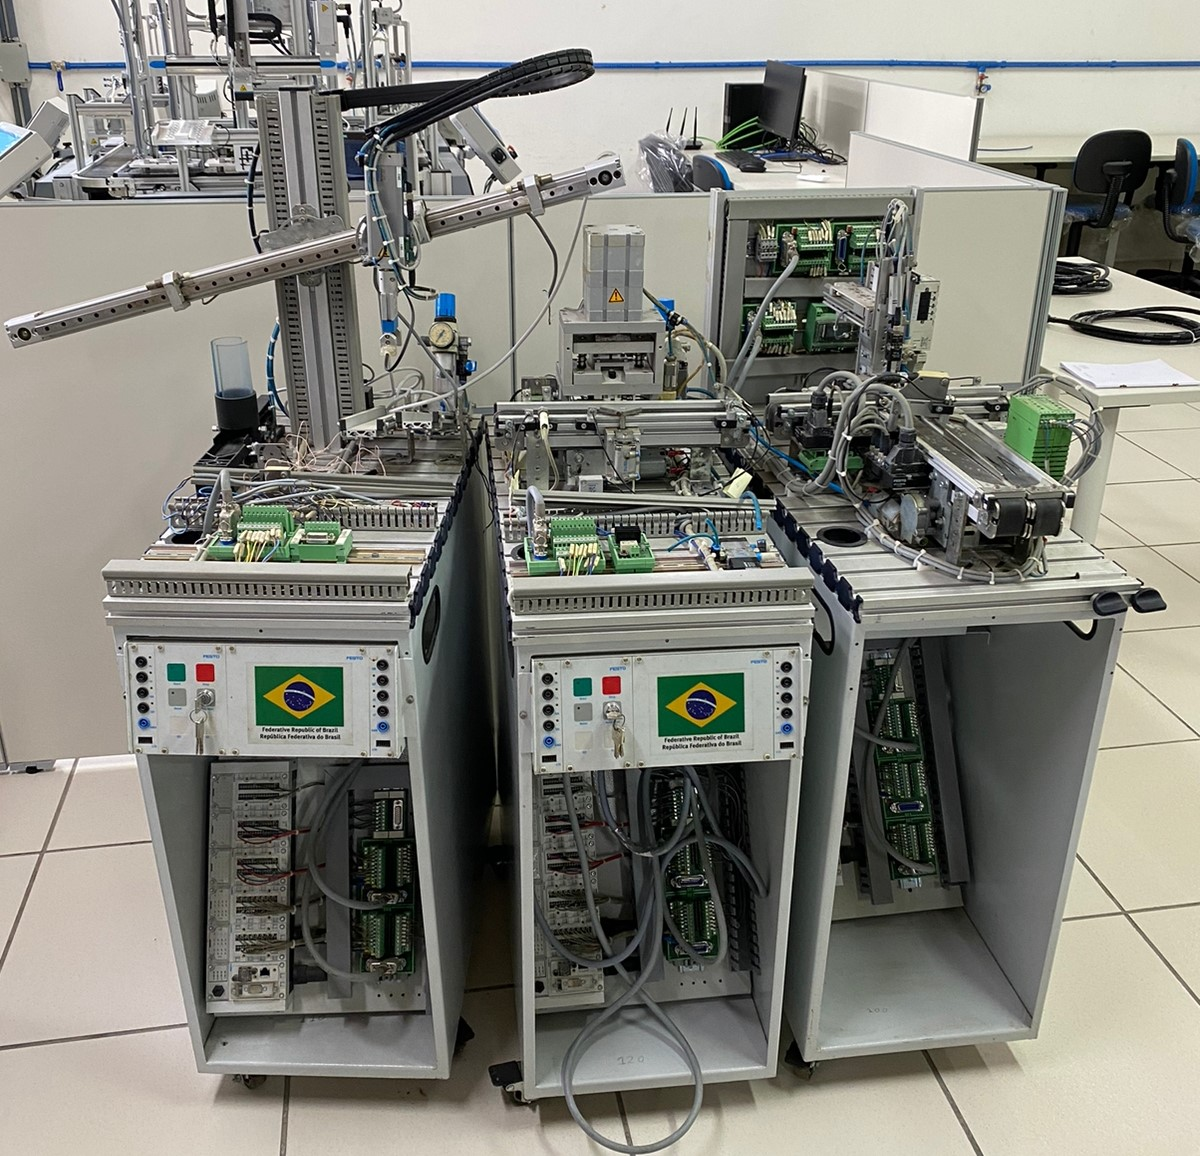
\includegraphics[width=0.93\linewidth]{figuras/mps_3mod.jpeg}
	\caption{Current status of the MPS platform}
	\label{fig:mps3mod}
\end{figure}

\begin{itemize}
\item \textbf{Transporter Module (\textit{Handling} - M1) -} the gripper's optical sensor was not properly fixed, the optical fibre and pneumatic hoses are deteriorated or broken, some electrical cables are disconnected, the entry pneumatic actuator was misaligned. The servo motor was functional, but its control driver had a partial electrical assembly, preventing the transporter from activating. The controller for this module, CPX-FEC PLC, was functional even though its control panel was not connected. The other electrical components are in good condition. Thus, the main requirements and limitations were identified, and the necessary activities and modifications for the proper update of the module, for the Industry 4.0 context, were identified to achieve the goals.

\item \textbf{Press Module (\textit{Press} - M2) -} The pneumatic hoses deteriorated, the pneumatic actuator for the conveyor was misaligned, the press piston was misaligned, and the pneumatic press actuator was misaligned. However, the sensors, controllers, and other electrical components are in good condition.

\item \textbf{Capper Module (\textit{Pick and Place} - M3) -} pneumatic hoses are deteriorated, and some electrical cables are disconnected; one functional conveyor and the other with a torn canvas; the control driver for the functional conveyance was operational; the positioning sensors are misaligned. 

The sensors are functioning correctly. The CPX-FEC PLC controller was also operational; however, the absence of the control panel was identified. Other components such as the suction cup and the pneumatic actuator for the Z-axis are worn out; however, components such as actuators and valves are in good condition and without leaks. The physical situation of this module was more complicated than that of the others. Several components need to be replaced or reinstalled to achieve proper updates in the context of Industry 4.0.

\item \textbf{Robotic Arm Module (\textit{Robot} - M4) -} integrates the platform with the stock. This module was not functional and has lost its home position. Due to the system being turned off for an extended period, the hoses deteriorated, and some electrical cables disconnected. The arm axes need lubrication, and the home and initial state points need re-calibration.

\end{itemize}

Similarly, after a brief test, it was observed that the robot controller turns on but does not initialize. The controller display does not light up, and on the Teach Pendant, only the initialization warning is signalled with an error code on the screen. There is also a Parts Storage Module (M5), which is used to allocate finished and/or discarded containers in the MPS platform process, and it is in good condition.

\subsubsection{Step 2 - Definition of the Objectives}

The proposed retrofit framework for the Modular Production System (MPS) platform is designed to restore, update, and connect the system with other devices. This enables synchronization with the Industry 4.0 framework, particularly in terms of technology that supports the digital twin concept.

This technique is especially useful in an academic setting, as it introduces and combines concepts essential to Industry 4.0. It serves as a platform for simulation and the development of new and existing operational proposals. Furthermore, it enables improvements and alterations to the process structure, as well as the commissioning of all stages.

The primary focus of the MPS platform's hardware update is the replacement of physical components, electrical and pneumatic connectors, and the updating of old technologies. The particular goals of this hardware update will be discussed in the following sections. 

The primary focus of the MPS platform's hardware update is the replacement of physical components, electrical and pneumatic connectors, and the updating of outdated technologies. The particular goals of this hardware update will be discussed in the following sections. By undergoing this update, the MPS platform is brought up to date with current concepts, improving its usability and performance following industry 4.0 requirements. The following are the detailed goals:

\begin{enumerate}
    
    \item Cleaning and sanitizing modules and components;
    \item Organization of electrical connectors;
    \item Replacement of all pneumatic hoses;
    \item Mechanical alignment of the conveyors in all modules;
    \item Calibration and testing of the pneumatic actuators in the modules;
    \item Replacement of module controllers with updated controllers;
    \item Replacement and installation of the optical sensor fibre in M1;
    \item The installation of a new motor and its respective driver in M1;
    \item Installation of a new acrylic protection in M2;
    \item Lubrication and calibration of the pneumatic actuator that inserts coins in M2;
    \item Replacement of the suction cup plunger for the caps in M3;
    \item Replacement of the belts on the conveyors in M3;
    \item Installation of the physical control panel for the module in M3.
\end{enumerate}

\subsubsection{Step 3 - Selection of Components and Technologies to be Updated}

The retrofitting process provides improved ease of use and configuration, the introduction of new functionalities, and the correction of any process concerns via web monitoring. Figure~\ref{fig:retrofit_atual} illustrates the result of the comprehensive approach applied to the Modular Production System (MPS) platform.

% The results include ease of use, configuration, the addition of new functionalities, and the correction of any process issues through web monitoring. Figure~\ref{fig:retrofit_atual} illustrates the outcome of the entire process applied to the MPS platform.

\begin{figure}[ht]
	\centering
	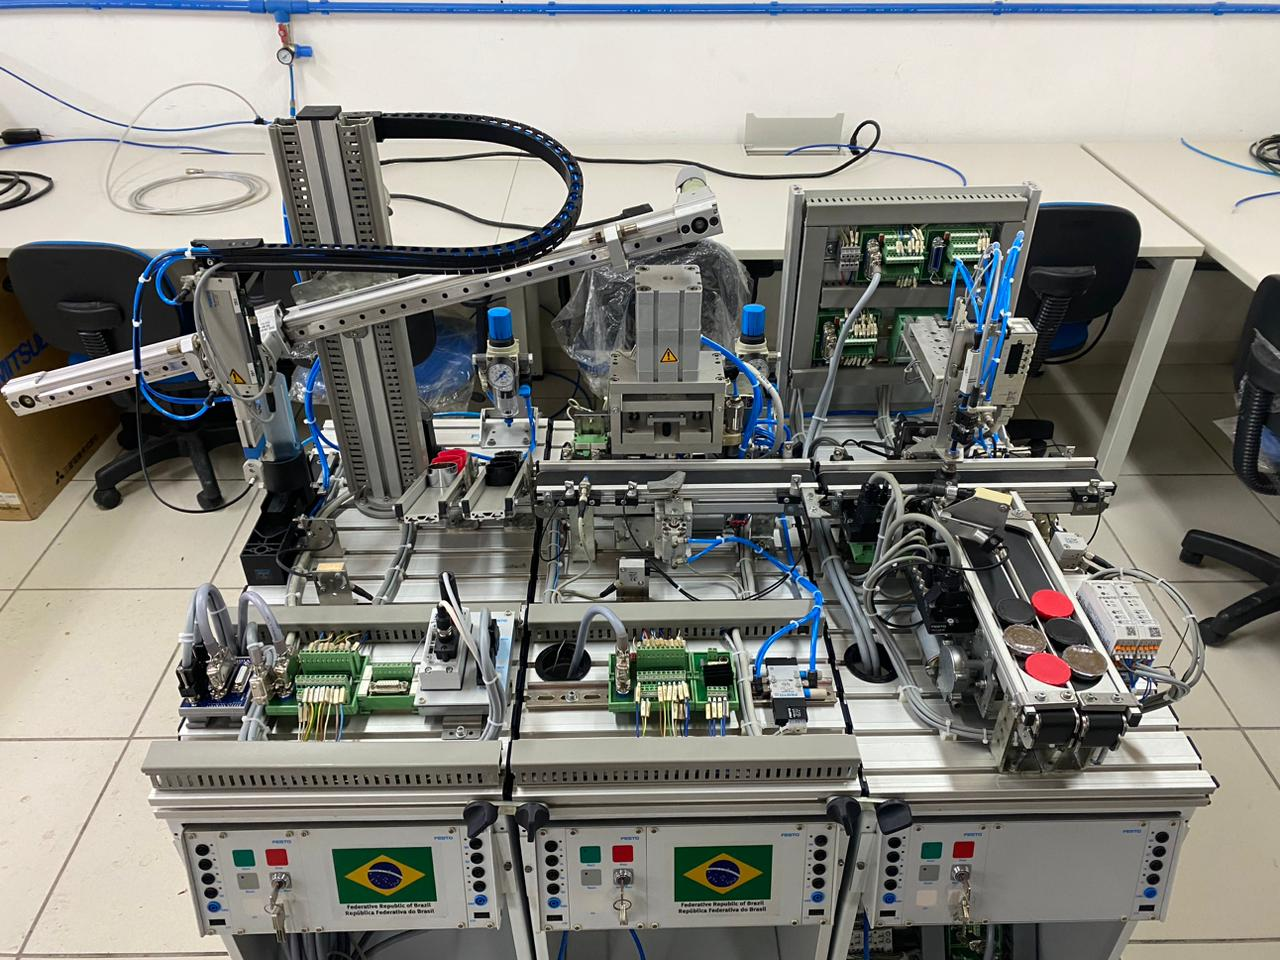
\includegraphics[width=0.99\linewidth]{figuras/mod_mps_atual.jpeg}
	\caption{Updated MPS platform }
	\label{fig:retrofit_atual}
\end{figure}

During the hardware updates, as shown in Table~\ref{tab:step3}, the new controller CPX-CEC-C1-V3 was installed. This controller was specifically built for controlling process systems. It is a small, high-performance device that combines automation operations, communication, and a human-machine interface in one device. It is powered by a high-speed microprocessor and has a variety of communication interfaces, including CANopen and USB.

\begin{table}[]
\caption{Selection to Updated System}
\label{tab:step3}
\begin{tabular}{l}
\hline
\multicolumn{1}{c}{\textbf{Updated System}} \\ \hline
CPU CPX-CEC-C1-V3                           \\
Switch with 08 gates TP-Link                \\
I/O Link / CANopen                          \\
Fieldbus node CTEU CANopen                  \\
PS control console for SysLink              \\
DC motor controller                         \\
I/O data cable, crossover, with socket      \\
FBA-2-M12-5POL                              \\
Access Point DIR-842                        \\
CODESYS V3, CIROS 7 and MES with licenses.  \\ \hline
\end{tabular}
\end{table}

This controller has an intuitive user interface that allows for simple process setting and monitoring. Its communication interfaces allow users to control a variety of automation devices, including actuators, sensors, and others. It is also used to monitor the status of devices and manage alarms and error messages. Programming tools that comply with IEC 61131-3 standards enable users to easily program and adjust the system's automated functionalities.

The CANopen network is an industrial communication network that uses the Controller Area Network (CAN) protocol. It was specifically designed to meet the communication requirements of industrial automation systems.

The CANopen network enables real-time monitoring and control of platform operations, as well as configuration and programming of various devices and modules. It provides a secure and effective method for assuring communication between various elements of a smart factory and enables the integration of various automation systems. The updated MPS system can function with increased communication and control thanks to the CANopen network, which is in line with Industry 4.0 requirements.

\subsubsection{Step 4 - Integration of New Components and Technologies}

This phase involves the integration and commissioning of new components and technology. This requires guaranteeing these components were appropriately incorporated into the existing system. The implementation was completed to generate a digital twin. 

An approach for connecting devices to the computer network using EasyPort was established. EasyPort is an interface that allows MPS platform modules to communicate with a computer via a USB connection. This interface provides a variety of tools for configuring and monitoring sensors and actuators involved in the process and is interoperable with a wide range of Festo components, including cylinders, valves, sensors, and actuators found on the MPS platform. It functions as a gateway, connecting one or more platform modules to the application, in this case, CIROS, where the digital twin was developed.

On the computer, in the CIROS Education, the digital twin was implemented to model, test, and train skills required for industrial production. Thus, the representation of the operation (virtual twin) of the MPS platform is implemented in the CIROS. It reveals features that provide real-time data monitoring, event logging, and remote diagnostics. This reproduction mirrors what is happening on the MPS platform (physical twin), the state of sensors and actuators, and the process status. Figure~\ref{fig:rep_real_virtual} shows how the physical twin's operation is replicated and synchronized with its virtual twin.

\begin{figure}[]
	\centering
	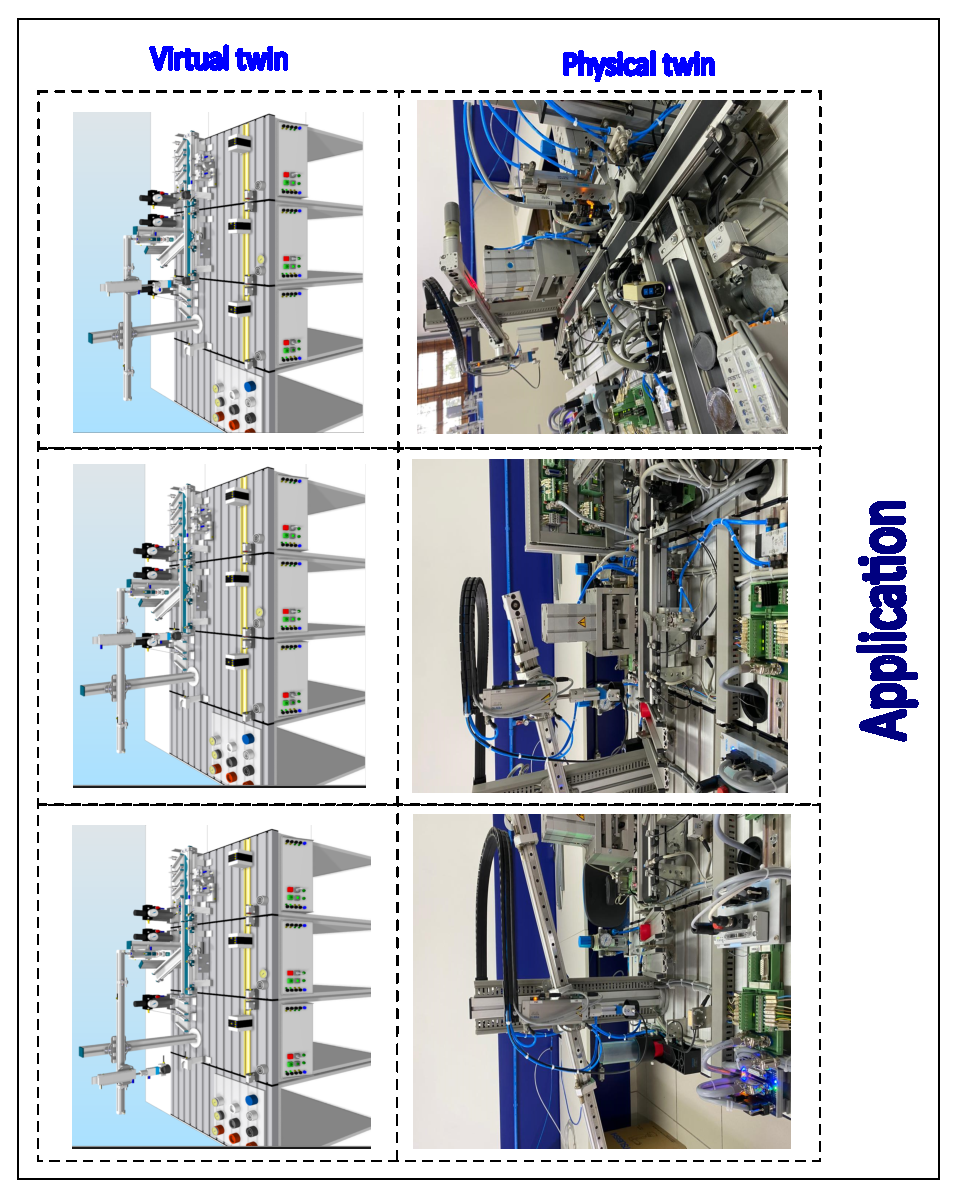
\includegraphics[angle=-90, width=0.9\linewidth]{figuras/result_all_3.eps}
	\caption{Digital twin application - reproduction of the operation of the physical twin and its synchronization with the virtual twin.}
	\label{fig:rep_real_virtual}
\end{figure}

Figure~\ref{fig:easy_atual} illustrates the process of obtaining the digital twin. The communication occurs via EasyPort and EZOPC, a connectivity interface that facilitates communication between Festo's automation equipment. EZOPC is a software tool that enables the communication and control of Festo components through an OPC (OLE for Process Control) connection, a widely used communication standard in the automation industry. OPC enables different control systems and devices to communicate effectively with each other.

\begin{figure}[]
	\centering
	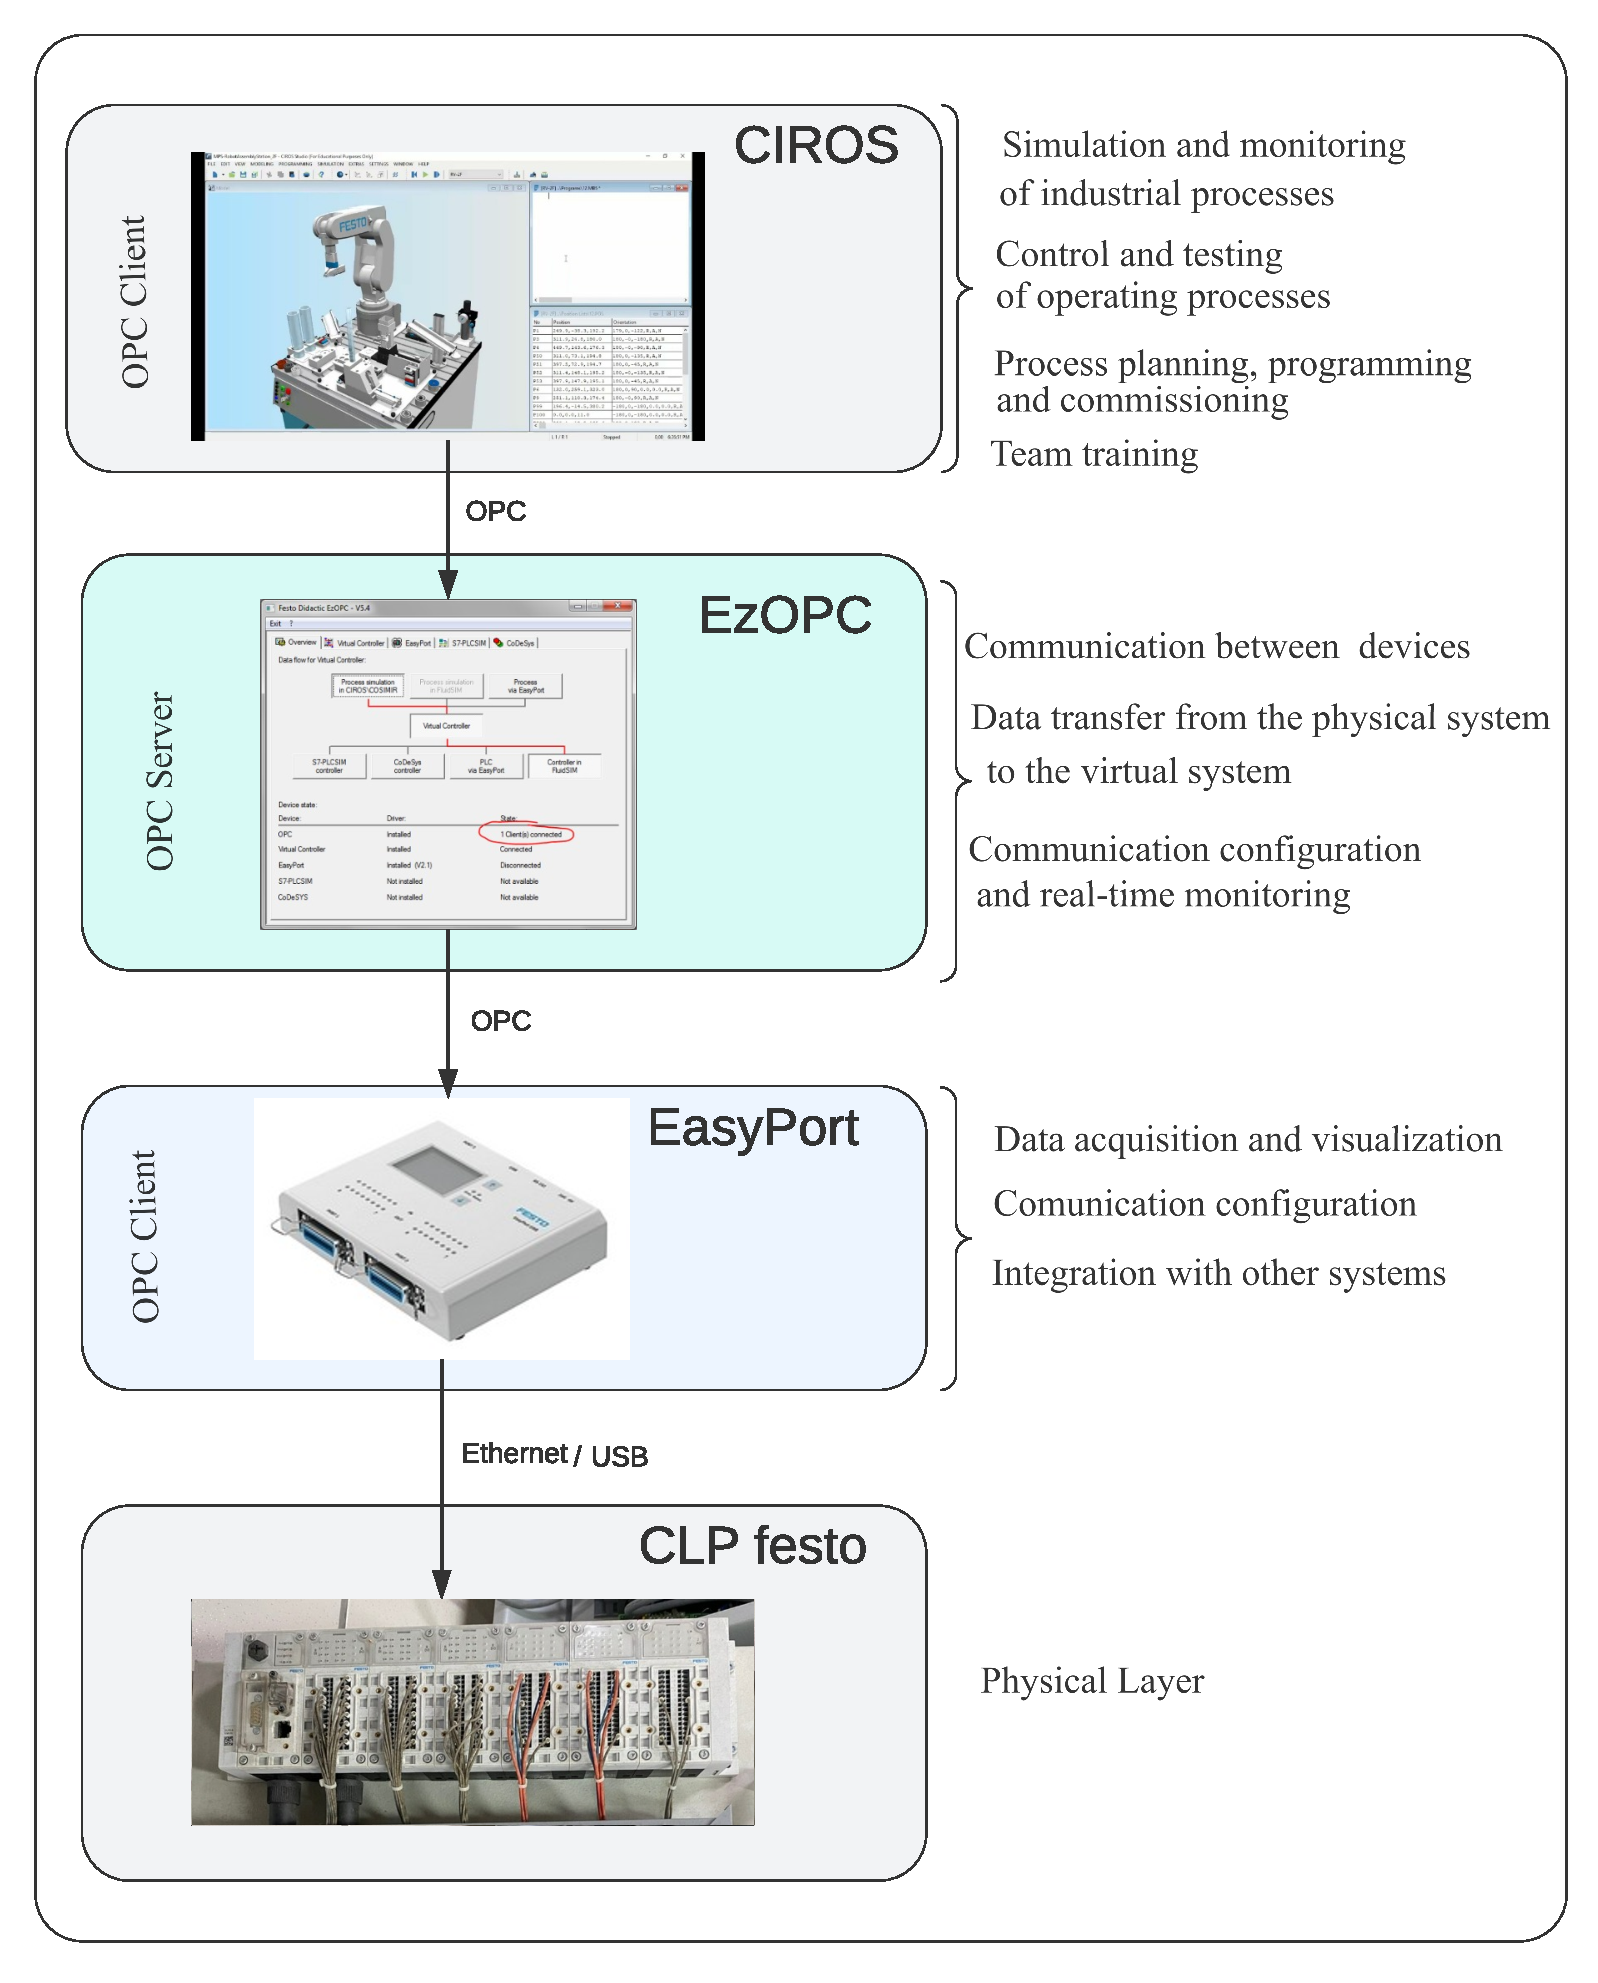
\includegraphics[width=0.9\linewidth]{figuras/d_easyport_result_eng.eps}
	\caption{Process of communication to achieve the digital twin}
	\label{fig:easy_atual}
\end{figure}

EZOPC functions as an OPC (OLE for Process Control) server, connecting the MPS (Modular Production System) platform's modules, which include various sensors and actuators, to external control systems such as PLCs (Programmable Logic Controllers) or SCADA (Supervisory Control and Data Acquisition). This arrangement enables seamless data exchange and control operations across several hardware and software platforms.

\begin{figure*}[ht]
	\centering
	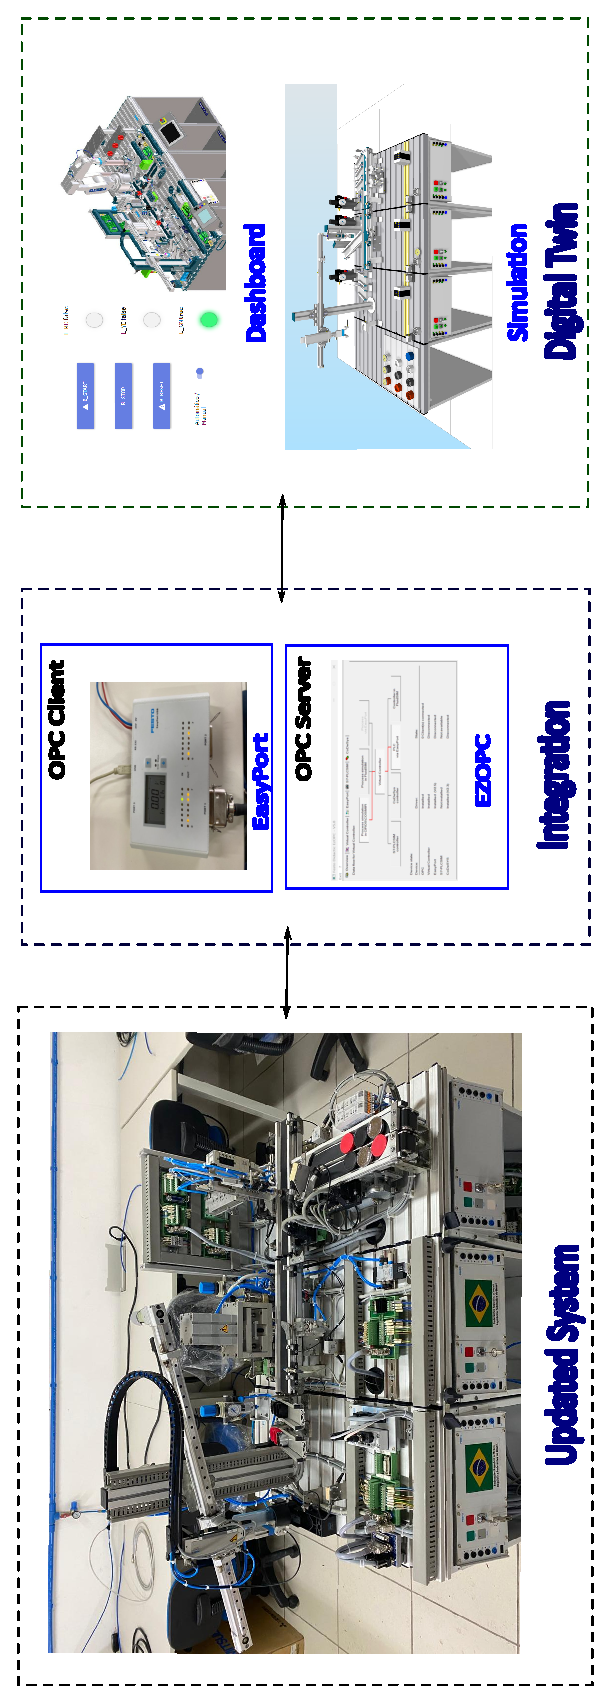
\includegraphics[angle=-90, width=0.99\linewidth]{figuras/result_all_5.eps}
	\caption{Final result obtained after applying the retrofitting methodology aiming to the digital twin }
	\label{fig:result_final}
\end{figure*}

In this configuration, CIROS operates as an OPC client. It communicates with EZOPC, the OPC server, via the OPC protocol. EZOPC, in turn, connects to EasyPort, another OPC client. This layered communication ensures that data from the MPS platform's sensors and actuators may be successfully monitored and controlled by other systems.

At the hardware level, the MPS platform is outfitted with updated modules that provide a variety of functionality and communication capabilities, both horizontally and vertically. Data is collected and transmitted via EasyPort to the digital twin program, which simulates and monitors the MPS platform's physical processes.

The integration and commissioning phases are essential for ensuring that all new components and technologies are smoothly integrated into the system. Throughout these phases, the system is rigorously validated and tested to improve its modelling, control, and data analysis capabilities. EasyPort and CIROS Education are used to construct a digital twin that simulates the physical processes of the MPS platform in a virtual environment. This complete strategy assures that the system functions safely, efficiently, and reliably.

Utilizing EZOPC as an OPC server, the MPS platform may successfully connect its modules to external control systems, allowing for enhanced monitoring and control. The integration of Industry 4.0 technologies and the production of a digital twin using tools such as EasyPort and CIROS Education greatly improve the system's capabilities, ensuring optimal performance and dependability.

\subsubsection{Step 5 - Testing and Validation of New Components and Technologies}

This step involves performing the production script and meticulously reviewing the system's performance, with an emphasis on the operation of actuators and sensors. These components are necessary for the MPS platform's accurate operation since they have a direct impact on manufacturing process control and monitoring. Furthermore, finishing and inspection tests are carried out to guarantee that the system satisfies all set quality standards.

It is important to ensure that all basic needs have been met during this phase. Any irregularities discovered must be corrected immediately. This may need revisiting the first steps (Steps 1 and 2) and redoing the full procedure to ensure complete integration and functionality. After making the necessary changes, the conformity of the new components and technologies may be validated, ensuring the system's safety, efficiency, and dependability.

The system has been tested through activation tests and operational cycles. These tests were created to ensure that the system performs optimally under a variety of scenarios. Figure~\ref{fig:result_final} shows that the proposed retrofit architecture was effective when applied to the MPS platform case study. The diagram depicts an intuitive interface for monitoring, configuring, and controlling processes in the physical twin.

During testing, the digital twin accurately duplicated the MPS platform's real-time activities. This involved monitoring actuator runtimes and detecting delays in the process, such as the pressing module, which took longer to accomplish jobs than other modules. The fundamental purpose of the digital twin was to replicate and control processes in real time. This functionality enables the interaction, pausing, and restarting of process parameters, allowing for detailed studies to assess the impact of changes and foresee probable undesirable situations in the MPS platform.

The proposed retrofit framework was verified by examining the smart factory's maturity level and product specifications. This complete method assures that the system operates with maximum safety, efficiency, and dependability. The extensive analysis and validation processes play an important role in determining whether the integration of new components and technologies improves the overall performance and reliability of the MPS platform.

By running the production script and doing detailed assessments, the system's actuators and sensors get checked to ensure they fulfill quality standards. Addressing any anomalies and certifying the system via activation tests and operational cycles ensures peak performance. The digital twin's capacity to mimic and control operations in real time expands the system's capabilities, making it a reliable solution for current production environments.

\section{Maturity level analysis considering the smart factory criteria}
\label{sec:results_2}

The maturity level of the MPS (Modular Production System) platform could be assessed to determine its alignment with Industry 4.0 technologies and practices. This study provides a thorough review of the system's features both as a legacy system and after retrofitting. The primary goal was for the improved MPS platform to perform significantly in the RAMI (Reference Architectural Model Industry 4.0) maturity assessment than when evaluated as a legacy system. This includes evaluating the maturity criteria for smart factories.

To classify the MPS platform based on smart factory and smart product maturity levels, each criterion's characteristics and degree of development were evaluated. The requirements for smart factories (F1-F5) were thoroughly evaluated. This evaluation allowed us to establish a reasonable classification for each parameter level.

This work makes a substantial contribution by evaluating and applying Industry 4.0 maturity levels and criteria. It is used to validate the suggested retrofit framework for the digital twin, which has been created throughout this research. The framework was guided by information gained from the initial review of the legacy system, which impacted the choice of components and technologies. This method resulted in a greater degree of development for each measured metric.

Table~\ref{tab:result_evaluation_factory} compares the legacy and updated systems using the smart factory criteria. The legacy system provided parameter F1 a level 3 based on the "good" level of automation achieved with electrical and pneumatic components. However, F2 was rated as level 2 because the MPS platform's integration was restricted by legacy architecture and interoperability problems.

\begin{table*}[]
% \begin{table}[]
\caption{Evaluation of the maturity level of smart factories}
\label{tab:result_evaluation_factory}
\begin{tabular}{|l|l|c|c|l|}
\hline
 &
  \multicolumn{1}{c|}{\textbf{Description}} &
  \begin{tabular}[c]{@{}c@{}}\textbf{Legacy System} \\ \textbf{Maturity level}\end{tabular} &
  \begin{tabular}[c]{@{}c@{}}\textbf{Updated System} \\ \textbf{Maturity level}\end{tabular} &
  \multicolumn{1}{c|}{\textbf{Smart factory criteria analysis}} \\ \hline
\textbf{F1} &
  Automation Process &
  Level 3 &
  Level 4 &
  \begin{tabular}[c]{@{}l@{}}\textbf{Legacy} - The classification of the legacy MPS platform as level 3 was based \\ on its satisfactory level of process automation. By utilizing electrical, hydraulic,\\ and pneumatic systems, this degree of automation is completed. Although these\\ systems offer a solid basis for automation, their real-time capabilities and\\ advanced functionalities are limited. \\ \textbf{Updated} - Following the retrofit framework, the updated MPS platform has advanced\\ to level 4. This update allows for more sophisticated automation of the process,\\ incorporating real-time control and monitoring capabilities. The integration of\\ advanced sensors and devices has significantly enhanced the platform's ability to\\ collect and process data efficiently. The improvements in system architecture\\ enable better interoperability and integration with other systems, thus supporting\\ a more flexible and responsive production environment. \end{tabular} \\ \hline
\textbf{F2} &
  System Integration &
  Level 2 &
  Level 4 &
  \begin{tabular}[c]{@{}l@{}}\textbf{Legacy} - The legacy MPS platform was classified at level 2 regarding its integration\\ capabilities. While it can be integrated with other systems, this integration is often\\ impeded by its outdated architecture. The legacy system architecture presents\\ challenges related to interoperability, which can limit the efficiency and \\effectiveness of coordinated control and data exchange with other systems. \\ \textbf{Updated} -  With the application of the retrofit framework, the updated MPS platform\\ has been elevated to level 4 in terms of system integration. This update facilitates\\ more efficient and seamless integration with other systems, enabling improved\\ coordination and control of the production process. The enhanced integration\\ capabilities were supported by modern communication protocols and advanced \\data management tools, which allow for real-time monitoring and control. \end{tabular} \\ \hline
\textbf{F3} &
  Intelligent Device Usage &
  Level 1 &
  Level 3 &
  \begin{tabular}[c]{@{}l@{}}\textbf{Legacy} - The legacy MPS platform was classified at level 1 because it does not\\ have integrated smart devices. While the system operates using basic automation\\ technologies, it lacks the advanced capabilities provided by smart sensors and\\ actuators. \\  \textbf{Updated} - Following the retrofit framework, the updated MPS platform has\\ advanced to level 4. This update enables more efficient system integration, allowing\\ for better coordination and control of the production process. The integration of\\ smart devices, such as advanced sensors and actuators, has significantly enhanced\\ the platform's capabilities. These smart devices facilitate real-time data collection\\ and analysis, improving decision-making processes and operational efficiency. \end{tabular} \\ \hline
\textbf{F4} &
  Data Analysis &
  Level 1 &
  Level 4 &
  \begin{tabular}[c]{@{}l@{}}\textbf{Legacy} -  The legacy MPS platform was classified at level 1 because it lacks\\ advanced data analysis capabilities. While the system can perform basic operations,\\ it does not have the integrated smart devices or sophisticated data processing tools\\ necessary for in-depth analysis. However, there is potential to enhance its\\ performance by integrating it with external data analysis systems. \\ \textbf{Updated} -  Following the retrofit framework, the updated MPS platform has advanced\\ to level 4. This update includes the integration of advanced data analysis capabilities,\\ allowing for more sophisticated analysis of production data. The system can now\\ identify trends and patterns that were previously undetectable, which helps optimize\\ the production process. Real-time data collection and analysis enable informed\\ decision-making, improving operational efficiency and responsiveness. \end{tabular} \\ \hline
\textbf{F5} &
  Production Flexibility &
  Level 2 &
  Level 3 &
  \begin{tabular}[c]{@{}l@{}}\textbf{Legacy} - The legacy MPS platform was classified at level 2 due to its certain degree\\ of production flexibility. This flexibility was achieved through the possibility of \\exchanging modules to change the type of product manufactured. However, this \\flexibility is somewhat limited by the legacy architecture and the fact that the modules\\ may have been designed to produce only specific types of products. \\ \textbf{Updated} - With the implementation of the retrofit framework, the updated MPS \\platform has advanced to level 3. This update, facilitated by tools such as CIROS,\\ allows for greater production flexibility. The updated system can now make real-time\\ adjustments and simulate different production scenarios, significantly enhancing its\\ ability to adapt to varying manufacturing requirements. \end{tabular} \\ \hline
\end{tabular}
% \end{table}
\end{table*}

The previous system's parameters F3, F4, and F5 were classed as level 1 because there were no intelligent devices installed or any capacity for data analysis and processing. The manufacturing method lacks flexibility due to intrinsic restrictions.

Following the update process, the findings revealed considerable improvements. Parameters F1, F2, and F4 achieved level 4, meeting requirements for enhanced automation, real-time process monitoring and control, increased integration, and efficient data gathering and processing capabilities. Parameters F3 and F5 attained level 3, indicating progress in process component improvements, flexibility, integration, and the ability to simulate various production scenarios.

The spider web graphic in Figure~\ref{fig:spider_all} demonstrates the success of the proposed retrofit architecture for digital twins. The graphic depicts significant improvements in the manufacturing process, including greater real-time data collecting and analysis, informed decision-making, and the identification of possible process concerns. Additionally, platform components' communication and connections were improved, making them more versatile and robust.

\begin{figure}[!t]
	\centering
	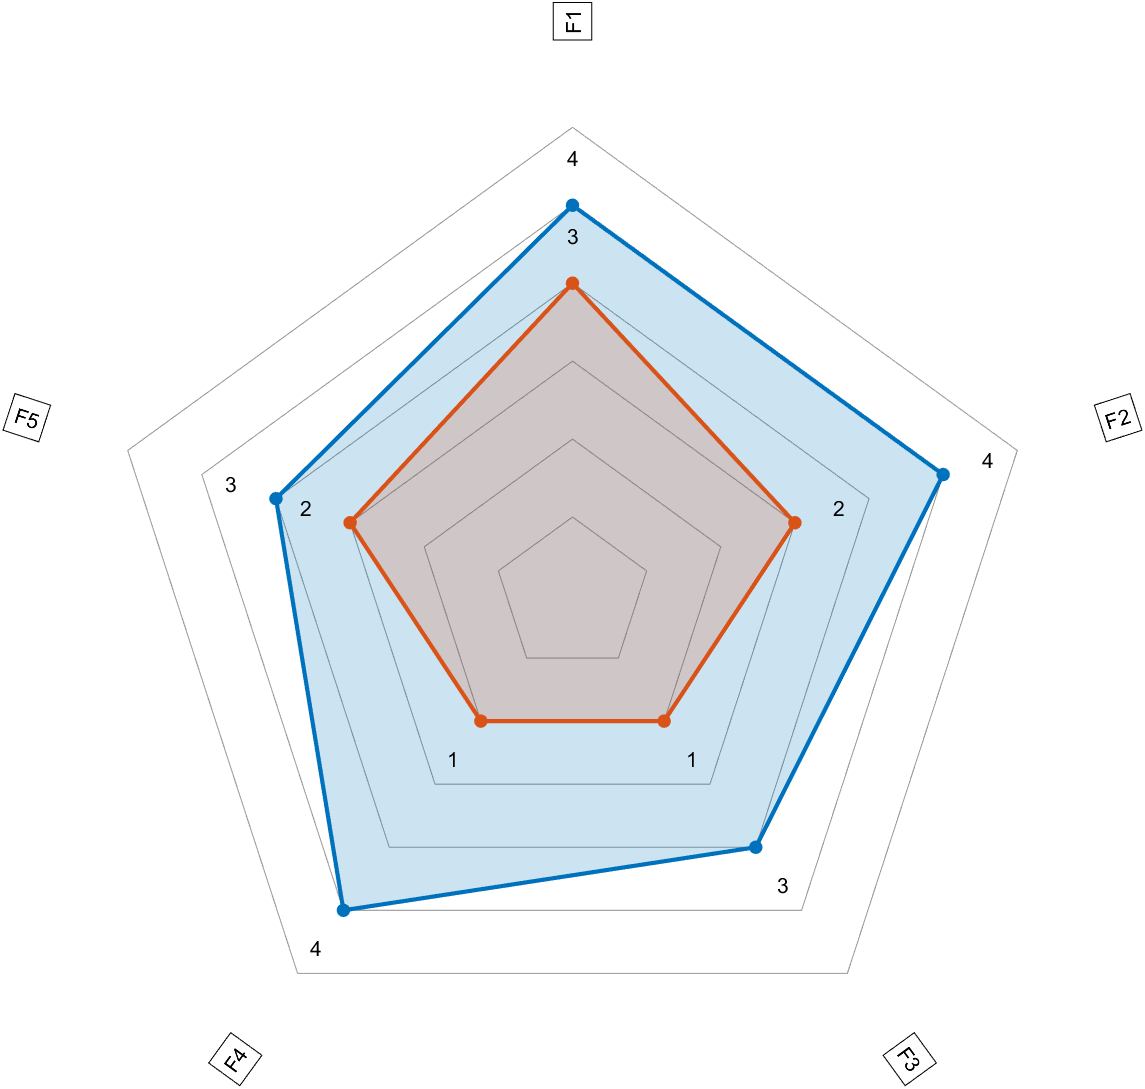
\includegraphics[width=0.99\linewidth]{figuras/grapf_final.png}
	\caption{Legacy System $\times$ Updated System}
	\label{fig:spider_all}
\end{figure}

Through studying and improving the maturity level of the MPS platform, the system's alignment with Industry 4.0 technologies and processes was greatly improved. The examination and application of Industry 4.0 criteria confirmed the suggested retrofit framework, resulting in significant gains in automation, integration, and data processing capabilities. The successful adoption of the digital twin highlighted the system's improved performance, flexibility, and dependability.

\section{Conclusion}
\label{sec:conclusion}

The proposed retrofit framework was applied to the MPS (Modular Production System) platform, to generate a digital twin, and the updated process improved significantly. Updates and replacements of sensors and devices on the MPS platform were executed following the defined systematic procedure, bringing the system up to Industry 4.0 requirements. This update brought various advantages, including a longer system lifespan, improved integration, flexibility, and others.

The evaluation of the MPS platform's maturity level, based on RAMI (Reference Architectural Model Industry 4.0) characteristics for smart factories, showed a considerable improvement from the legacy to the updated system. The goal of a higher position in the maturity evaluation demonstrates the dedication to aligning the MPS platform with the most recent industry trends and practices.

The most notable contribution of this work is the effective implementation of the retrofit framework aimed at the digital twin. The validation of the technique through the evaluation of the Industry 4.0 maturity level emphasizes the need for retrofitting and aligning modernization practices with evolving industry demands. This technique not only verifies the retrofit architecture but also emphasizes the strategic value of updating legacy systems to meet modern requirements.

The table and spider web chart provide a comparative examination of the legacy and updated systems, which supports the retrofit's success. The investigation identifies significant gains in some critical areas, including real-time data gathering and analysis, informed decision-making, process integration and interoperability, and improved communication among platform components. The use of communication and simulation tools such as CANOpen, EasyPort, EZOPC, and CIROS was essential to the update process, allowing for more efficient integration while also matching the basic methodology requirements.

\bibliographystyle{IEEEtran}

\bibliography{mybibfile.bib}

\end{document}


